\chapter{\IfLanguageName{dutch}{Stand van zaken}{State of the art}}
\label{ch:stand-van-zaken}

% Tip: Begin elk hoofdstuk met een paragraaf inleiding die beschrijft hoe
% dit hoofdstuk past binnen het geheel van de bachelorproef. Geef in het
% bijzonder aan wat de link is met het vorige en volgende hoofdstuk.

% Pas na deze inleidende paragraaf komt de eerste sectiehoofding.

De stand van zaken verduidelijkt de hedendaagse problemen en bezorgdheden in de wereld van de mainframe. Aan de hand van een literatuurstudie worden deze problemen in kaart gebracht.

\section{\IfLanguageName{dutch}{Het verdwijnen van expertise}{Lostage of expertise}}
\label{sec:Verdwijnen van expertise}

Veel informatietechnologiespecialisten, zoals Stewart Alsop, voorspelden dat de stekker uit de laatste mainframe zou worden gehaald aan het einde van de jaren 90 \autocite{McCracken2012}. Volgens het onderzoek van \textcite{Waites2013} zal de mainframe nog niet verdwijnen, maar de expertise wel. Mainframe-applicaties die cruciaal zijn voor de werking van bedrijfsprocessen, zorgen voor een angst dat de complexe expertise voor het ontwikkelen en onderhouden van deze applicaties aan het verdwijnen is. De mainframe-ontwikkelaars die geboren zijn tussen 1945 en 1964 zijn gepensioneerd of gaan op pensioen. Dayton Semerjian zei in het artikel van \textcite{Waites2013}: ``The average age of mainframe workers is 55 to 60''. Veel organisaties zien outsourcing van hun workloads als een oplossing voor de tekorten aan experten. Dat is een manier waarop ze een compensatie proberen creëren om hun mainframe workloads te behouden en tegelijkertijd te onderhouden en verbeteren. Het problematisch aspect hierbij is dat het heel tijdrovend en vermoeiend is voor een organisatie om de benodigde kennis door te geven. Aan de hand van technische kennis is er volgens \textcite{Waites2013} bij mainframe-ontwikkeling heel wat te doen, echter is kennis over de organisatie eveneens van groot belang.


In 1960 ontwikkelden dr. Grace Hopper en haar collega's de programmeertaal COBOL. Deze programmeertaal is naar schatting gegroeid van 150 tot 250 miljard lijnen applicatiecode, waarvan acht tot negen miljoen nieuwe lijnen per jaar worden bijgeschreven \autocite{Waites2013}. Het is volgens \textcite{Waites2013} nog steeds de populairste programmeertaal in de mainframewereld. Daarentegen met de ontwikkeling van andere programmeertalen, wordt COBOL afgeschreven als 'out-of-date' en 'dying'. Elk jaar sinds 1970 werd het uitsterven van COBOL een volkomen zekerheid. Als een organisatie een mainframe heeft, zijn de kansen zeer groot dat al hun applicaties geschreven zijn in COBOL \autocite{Waites2013}. 

Het was waarschijnlijk dat programmeurs die in de jaren 70 en 80 in de technologiesector stapten, COBOL-programmeurs werden. Daarom is het duidelijk dat de leeftijd van mainframe-experten verschillend is van de leeftijddistributies die in de UNIX- en Windowsomgevingen plaatsvindt \autocite{McGirr2004}. Volgens studies van Meta Group zijn 60\% van de mensen die werken op een mainframeomgeving  50 jaar of ouder in vergelijking met de 8\% in een UNIX- of Windowsomgeving. Slechts 5\% zijn onder de 30 jaar. Hieruit concludeert  \textcite{McGirr2004} dat veel mainframe-experten de pensioenleeftijd naderen. 

In het verleden werden veel IT-professionals geïntroduceerd in de informaticasector door te programmeren. Veel universiteiten boden COBOL-cursussen aan in mainframeomgevingen. Met het opkomen van nieuwe en modernere programmeertalen begonnen universiteiten deze cursussen uit te dunnen of zelfs te schrappen uit hun curriculum  \autocite{Mullins2016}. Hierdoor verloor de programmeertaal COBOL zijn populariteit. Studenten voelden zich meer aangetrokken tot de meer moderne en aantrekkelijke programmeertalen zoals Java en C++. Veel jonge IT-professionals zien het niet meer zitten om op mainframesystemen te werken \autocite{Mullins2016}. Het groene 3270-terminalvenstertje is niet het meest aantrekkelijke in vergelijking met omgevingen zoals Eclipse, Visual Studio en Visual Studio Code. Wat de meeste jonge IT-professionals niet weten, is dat het niet meer de norm is om enkel in dat groene terminalvenstertje te werken. 

De moderne mainframe is heel verschillend ten opzichte van wat de meeste studenten of IT- professionals denken. Mainframes kunnen al sinds 1960 makkelijk gekoppeld worden via de parallel sysplex technologie. Dat is een clusteringtechnologie die toelaat om verschillende kopieën te hebben van het z/OS besturingssysteem in één enkele image. Deze technologie biedt de mogelijkheid om meerdere systemen te laten werken en toch hun data over alle systemen te kunnen raadplegen en gebruiken \autocite{Sarkar2020}. Daarnaast is het mogelijk om moderne technologieën zoals Linux- en Windowsplatformen te gebruiken op een mainframe. Dat wil zeggen dat Java, XML, TCP/IP enzovoort bruikbaar zijn. De oorzaak van deze onwetendheid is het gebrek aan kennis en het opleidingsaanbod \autocite{Mullins2016}. Volgens \textcite{Mullins2016} wordt mainframetechnologie niet meer aangeleerd door universiteiten en/of hogescholen, wat zou moeten veranderen. Maar zal het veranderen? De naam van de mainframe zou aantrekkelijker kunnen gemaakt worden om ervoor te zorgen dat deze technologie terug de nieuwe generatie IT-professionals aantrekt. \textcite{Mullins2016} vond de naam AlwaysAvailable een passende naam.


Volgens het artikel van Open Mainframe Project \autocite{2020} zijn er 4300 instellingen in de Verenigde Staten waar het mogelijk is om een diploma te verkrijgen. Slechts 10 tot 15 instellingen bieden een semestriële cursus aan die te maken heeft met een mainframe. De reden die zij hiervoor aangeven is het feit dat een tekort aanwezig is aan facultatieve kennis om deze cursussen aan te bieden. Mainframe-experten zouden hun kennis opgedaan hebben on the job en niet meer via hun opleiding. Dat zorgt ervoor dat het hoger onderwijs niet toelaat dat deze personen hun kennis doorgeven op academisch niveau \autocite{2020}. 

\section{\IfLanguageName{dutch}{De laatste nieuwe mainframe technologie}{The most recent mainframe technology}}
\label{sec:De laatste nieuwe mainframe technologie}

Er wordt wel eens gezegd dat de mainframe dood is. De mainframe is over de jaren heen al vele keren dood verklaard. Toch wordt de 'Big Iron' meer en meer gemoderniseerd. De nieuwste generatie mainframe van IBM heeft bewezen dat de mainframe nog sterk aan innovatie onderheven is \autocite{Almekinders2022}. Volgens IBM zullen mainframes nog zeker deel uitmaken van de hedendaagse informatica en dat bewezen ze met de IBM z16. Deze nieuwe mainframe bevat een Telum-processor. Hierop bevindt zich een accelerator met AI-inferencing. Dergelijke systemen bieden klanten tijdige, geïnformeerde en aangepaste oplossingen om beslissingen te helpen maken terwijl ze tegelijkertijd geschikte beveiligingsmechanismen voor AI-modellen gebruiken \autocite{Cammarota2020}. In het geval van de z16, belooft IBM dat dit realtime AI toevoegt aan workloads die op een dergelijke mainframe gedaan worden. Via de Telum-processor kunnen banken fraude detecteren tijdens transacties op grote schaal. Als gevolg hiervan voorkomt de realtime AI dat klanten en/of bedrijven grote verliezen maken vanwege frauduleuze praktijken. De z16-mainframe kan met behulp van artificiële intelligentie ervoor zorgen dat de kans op fraude significant wordt verkleind. Fraude zou opgemerkt en gesignaliseerd kunnen worden nog voor de transactie volbracht is \autocite{Saran2022}. Hiermee zetten zij in op maximale security van transacties. Dat zonder impact op de Service Level Agreements (SLA). Een service level agreement of SLA definieert het servicelevel dat de klant verwacht van de fabrikant of leverancier van diensten of producten. Volgens bepaalde criteria wordt een doelstelling van tevredenheid over de dienst of product vastgelegd, waar vervolgens een akkoord wordt over gesloten. Zo wordt verwacht dat de nieuwe mainframe de pure prestaties behoudt om aan de verwachtingen van hun klanten te voldoen. Banken en verzekeringsinstellingen kunnen dezelfde latency verwachten, echter met artificiële intelligentie bovenop \autocite{Saran2022}. AI-inferencing maakt het mogelijk voor financiële instellingen om transacties sneller en efficiënter af te handelen. Een praktisch voorbeeld waarbij AI-inferencing nuttig kan zijn is het versnellen van de afsluitingen van leningen en het bepalen van transacties met hogere risico's \autocite{Saran2022}.


\subsection{\IfLanguageName{dutch}{Quantum computing en IBM Z16}{Quanting computing and IBM z16}}
\label{sec:Quantum computing en IBM z16}

IBM speelt een grote rol in de wereld van quantum computing. De ontwikkeling van deze vrij nieuwe technologie heeft ook een donkere zijde. Veel cryptografiemethodes kunnen eenvoudig worden doorbroken door quantum gebaseerde gevallen. Denk hierbij aan het uitwisselen van walletkeys of digitale handtekeningen. De wiskundige methodes die deze zaken gebruiken zijn eenvoudig op te lossen met een quantumcomputer. Volgens Anne Dames, Distinguished Engineer, Cryptographic Technology Development Systems bij IBM wordt het aanvalsoppervlak van systemen en organisaties met quantum computing een stuk vergroot \autocite{Almekinders2022}. Natuurlijk moet de IBM z16 dat probleem tegengaan. De nieuwe mainframe maakt gebruik van lattice-based cryptografie. Volgens \textcite{Almekinders2022} is het mogelijk om wiskundige probleemstellingen te creëren die zelfs quantumcomputers niet kunnen oplossen. 

\section{\IfLanguageName{dutch}{IBM Mainframe modernisatie}{IBM Mainframe modernization}}
\label{sec:IBM Mainframe modernisatie}


\subsection{\IfLanguageName{dutch}{Workloads migreren naar de cloud - Google Cloud Platform}{Migrating workloads to the cloud - Google Cloud Platform}}
\label{sec:Workloads migreren naar de cloud}


Google Cloud is een uitstekende keuze als het gaat om een omgeving waar een IBM z/OS mainframe workload naar zou kunnen migreren \autocite{Astadia2021}. Dat platform biedt gelijkaardige securitylevels en de mogelijkheid om te kunnen schalen naar wat de gebruiker ervan verwacht. Het biedt enerzijds ook een omgeving die z/OS mainframe legacy ondersteunt dat reeds migreerde naar de cloud. Volgens \textcite{Astadia2021} zijn het aantal personen dat de skills beheersen om mainframe legacy te onderhouden aan het dalen en worden zij niet vervangen. Anderzijds stijgen hardware- en softwareonderhoudskosten continu om te kunnen voldoen aan de innovatieve eisen die veel klanten hebben. Innovatieve eisen die IBM z/OS mainframe platformen niet kunnen bieden. 

\subsection{\IfLanguageName{dutch}{Wat is Astadia?}{What is Astadia?}}
\label{sec:Wat is Astadia?}

Sinds 1994 is Astadia één van de grootste uitdagingen op vlak van modernisatie, cloudmigratie, replatformering en applicatiemodernisatie aangegaan. Zij zijn wereldleider in high-performance mainframe modernization. Astadia begeleidt organisaties om een transformatie roadmap op te stellen om weg te migreren van hun mainframe legacy. 

\subsection{\IfLanguageName{dutch}{Waarom zou de mainframe legacy gemigreerd worden naar Google Cloud?}{Why should we migrate our mainframe legacy to Google Cloud?}}
\label{sec:Waarom zouden we onze mainframe legacy en databases migreren naar Google Cloud?}

Volgens \textcite{Astadia2021} is het kostenplaatje van een mainframe al een interessante factor om een migratie te overwegen. De Total Cost of Ownership (TCO) van een platform zoals Google Cloud zou op een korte termijn van 12 maanden al een aantrekkelijke Return On Investment (ROI ) geven in vergelijking met IBM z/OS mainframe. Daarnaast beweren zij eveneens dat de mensen met de juiste skills aan het verminderen zijn en niet vervangen worden. Het aanbod van IT-professionals met de nodige kennis en expertise verdwijnt \autocite{Astadia2021}. Google Cloud daarentegen is een aantrekkelijker en meer populair platform dat wereldwijd meer jonge IT-professionals naar zich toe trekt. Ten slotte speelt de flexibiliteit volgens \textcite{Astadia2021} een grote rol. Volgens hen is Google Cloud meer flexibel op vlak van het schalen van businessvereisten. Het ondersteunen van een groot aantal gebruikers en toestellen zou beter tot zijn recht komen, net als database sharing. 

Er wordt in dit onderzoek vaak gesproken van moderniseren of migreren. Toch zijn deze termen geen synoniemen. Migreren is een type van modernisatie. Migratie houdt ook andere zaken in zoals replatform, refactor, rewrite en replace processen. Replatform is een proces dat bestaande code in COBOL of in PL/1 van de mainframe haalt. Deze code zal dan gecompileerd en uitgevoerd worden in een z/OS-emulator die draait op Google Cloud. Dat is een manier om tijd en geld te besparen. Indien alle bestaande legacy code moet herschreven worden, kost dat veel tijd en de juiste mensen om dat te verwezenlijken. IBM z/OS applicaties gaan draaien op een gehoste emulator door Google Cloud. Dat brengt de mogelijkheid met zich mee om API's te voorzien voor eerder ontoegankelijke programma's en data. Vaak is het wel zo dat de  mainframeapplicatiecode eerder omgevormd wordt naar Java of C\#. Deze programmeertalen zijn object georiënteerd, wat beter past bij de aard van cloudgebaseerde applicaties. Dat staat bekend onder het proces refactor \autocite{Astadia2021}. Natuurlijk is de enige praktische en efficiënte manier om dat te doen door het proces te automatiseren om mainframeapplicatiecode bijgevolg te transformeren. Als voorlaatste proces binnen een migratie naar de cloud is er rewrite. Hierbij worden nieuwe programma's ontwikkeld om de IBM z/OS mainframe te moderniseren. Vaak is dat riskant en het meeste van de pogingen om programma's te herschrijven mislukken. Het is te complex met een hoog kostenplaatje. Een betere aanpak is om de applicatie te verplaatsen naar een Google Cloud gebaseerde emulator. Dat houdt in dat er ook gemigreerd wordt naar een Google Cloud gebaseerde databank waarbij de focus ligt op het vervangen van modules en code in verschillende fases. Als het tijd is om aan rewrite te doen, zijn transformatie-engines vaak de beste optie met een zo laag mogelijk risico. Als laatste proces in de migratie naar Google Cloud is er het replace proces. De bedoeling hiervan is om de functionaliteit van de mainframe te vervangen door een programma of een verzameling van programma's. Dat is een typische Software-as-a-Service-applicatie (SaaS) \autocite{Astadia2021}. 

\subsection{\IfLanguageName{dutch}{De uitdagingen van mainframemodernisatie volgens Astadia}{De challenges of mainframe modernization according to Astadia}}
\label{sec:De uitdagingen van mainframemodernisatie volgens Astadia}

In de informatietechnologie, met name software development, is het aangewezen om documentatie over een bepaalde applicatie of stuk software bij te houden. Dat is echter niet altijd zo geweest. In de vroege jaren van commerciële mainframe computing werd dat nooit gedaan  \autocite{Zachry2001}. De ontwikkelingen rond softwaredocumentatie begonnen rond deze tijd pas onder stoom te komen. Dat sluit ook meteen aan bij de uitdagingen die volgens Astadia op de weg liggen bij een mainframemodernisatie. Veel IBM z/OS mainframeomgevingen vertrouwen dagelijks op honderden applicaties en transacties waar geen documentatie voor bestaat waarin beschreven staat wat ze doen \autocite{Zachry2001}. In veel gevallen zijn applicaties op mainframe al enkele decennia oud. Daarnaast hebben veel van deze applicaties dependencies of afhankelijkheden binnen het systeem om hun taak te doen. Denk maar aan een Db2 databank of een groep van sequentiële bestanden. Als deze dependencies niet gedocumenteerd zijn, is het moeilijk om te achterhalen wat deze applicaties nodig hebben tijdens hun uitvoering \autocite{Zachry2001}. Om een succesvolle migratie door te voeren is het van essentieel belang dat de dependencies mee gemigreerd worden met de applicatie. Anderzijds is er een uitdaging die te maken heeft met het draaien van parallelle systemen. Bij sommige IBM z/OS mainframe applicaties is het nodig om aan parallelle verwerking te doen. Deze applicatie is dan nog steeds in gebruik in de productieomgeving en tegelijk op het nieuwe platform. De planning en de uitvoering voor deze processen is een uitdaging die hoort bij de migratie van een IBM z/OS mainframesysteem. Er moet eveneens rekening gehouden worden met de integriteit van data \autocite{Astadia2021}. Het migreren van een grote databank naar een nieuwe doeldatabank vereist een reorganisatie en ordening van de oude data. Dat is nodig om de integriteit van data te bewaren. 

Hieruit concludeert \textcite{Astadia2021} dat het een goed moment is om een validatie uit te voeren van de organisatiedata bij een migratie. Het kostenplaatje is vaak een achilleshiel in de migratie van het IBM z/OS platform naar een Google Cloud omgeving \autocite{Astadia2021}. Organisaties hebben bij het moment van een migratie een dubbele kost die zij moeten betalen. Zij betalen voor het in stand houden van de productieomgeving die draait op een mainframe. Daarnaast steken zij alle moeite en geld in de migratie naar het nieuwe systeem. Dat heeft een tijdelijk financiële impact op de welvaart van een organisatie waar rekening mee moet worden gehouden \autocite{Astadia2021}. 

Ten slotte is de expertise rond het migreren tijdens een migratie van heel groot belang. Het is een vereiste dat zowel expertise aanwezig is op vlak van de organisatiestructuur als technische kennis van de nieuwe programmeertalen, databanksystemen, netwerken en vele andere componenten. Alle workloads die migreren naar Google Cloud moeten dezelfde functionaliteit bewaren als voordien. Hierdoor is het belangrijk dat de functionele analisten binnen de migratieplannen een gedetailleerd ontwerp uittekenen dat alle use cases in kaart brengt van de oude mainframeapplicaties. Het einddoel is dat het Google Cloud platform werkt zoals het IBM z/OS mainframe platform door het iteratief en consistent uitvoeren van testen \autocite{Astadia2021}. 

\subsection{\IfLanguageName{dutch}{De voordelen van migreren naar Google Cloud volgens Astadia}{De benefits of migrating to Google Cloud according to Astadia}}
\label{sec:De voordelen van migreren naar Google Cloud volgens Astadia}

Volgens \textcite{Astadia2021} is het makkelijker om Google Cloud te gebruiken dan het IBM z/OS mainframe platform. Google Cloud is ontworpen met eenvoudigheid als uitgangspunt. Het is mogelijk om nieuwe services en applicaties te hosten door het gebruik van de ``web-based Google Cloud Management Console ``.  Er is veel meer documentatie beschikbaar en online informatie op forums en websites. Het is daarnaast een flexibeler systeem, omdat het mogelijk is om een groot aantal virtuele omgevingen te kiezen die het best bij de workloads passen en die overeenstemmen met de vereisten van de applicaties. In het geval dat er geen adequate omgeving wordt gevonden, kan er simpelweg een ander type instantie worden voorzien. 

Google Cloud is beter op vlak van prijs en kwaliteitsverhouding volgens \textcite{Astadia2021}. Een bedrijf betaalt enkel voor de resources die ze gebruiken zonder vastliggende contracten of verplichtingen. Bij het gebruik van een IBM z/OS mainframesysteem hebben organisaties een hoge verwachting op vlak van betrouwbaarheid, veiligheid en snelheid. Google Cloud biedt volgens \textcite{Astadia2021} een wereldwijde computerinfrastructuur die al deze factoren evenaart. Google Cloud biedt daarnaast meerdere security capabilities en services  die privacy verbeteren. Deze omvatten Google Cloud Virtual Private Cloud (VPC), die private of dedicated netwerkconnecties encrypteert. 

\subsection{\IfLanguageName{dutch}{Is een IBM z/OS mainframeworkload een goede kandidaat voor migratie naar een publieke cloudomgeving?}{Is a IBM z/OS mainframe workload a good candidats for migration to public cloud environment?}}
\label{sec:Welke workloads kunnen gemigreerd worden naar de cloud?}

Een publieke cloud is een platform dat gebruik maakt van een standaard cloud computing model om resources beschikbaar te stellen voor cloudcomputing \autocite{Allison2016}. Typische IBM z/OS mainframe workloads, waaronder COBOL, PL1, CICS en IMS, zijn geen geschikte workloads om naar een publieke cloudomgeving te migreren. De reden hiervoor is de besturingssysteemomgeving. De controle of een workload geschikt is gebeurd op basis van verschillende criteria. Veronderstel dat de workload een geschikte kandidaat is voor een migratie naar een cloudomgeving, dan is de volgende stap om na te denken over de opslaglagen. Een voorbeeld van een opslaglaag is de cloud, echter heeft een workload altijd meerdere lagen. Deze worden bepaald aan de hand van prestaties, I/O-capaciteit, beschikbaarheid en schaalbaarheid \autocite{Allison2016}. Volgens het onderzoek van \textcite{Martikainen2018} zijn er geen duidelijke karakteristieken waar een mainframe workload moet aan voldoen om te migreren naar de cloud. Organisaties hebben verschillende soorten applicatiearchitecturen op hun mainframe. Daardoor varieert de complexiteit van de bestaande applicaties door de onderliggende architecturen. \textcite{Orban2016} stelt voor om hierover na te denken op basis van een spectrum van complexiteit. De gevirtualiseerde service-georiënteerde architectuur zou aan de lage complexiteit van het spectrum liggen en de monolitische mainframe aan de hoge complexiteit van het spectrum. Volgens hem zou het starten aan de lage complexiteit van het spectrum makkelijker te volbrengen zijn bij een migratie, waardoor de kans op slagen groter zou zijn \autocite{Orban2016}. 

Er wordt best eerst gefocust op de minst complexe of strategische applicaties \autocite{Korzenlowski2017}. Dat zijn applicaties die gebruikers nodig hebben om hun werk uit te voeren of die essentieel zijn voor de organisatie. Volgens \textcite{Marble2017} zijn mainframeworkloads en architecturen uitermate complex. Het feit dat mainframes duizende transacties kunnen verwerken per seconde spreekt voor zich. Er is nood aan een perfecte planning om mainframeworkloads te migreren naar open systemen \autocite{Marble2017}. De eerste stap in een migratieplan is om volgende aspecten in de workload te bekijken:
    \begin{itemize}
        \item Omgevingen
        \item Applicaties
        \item Databanken
        \item Packages
        \item Utilities
        \item Tests
        \item Gebruikers
        \item Programmeertalen
    \end{itemize}
Vervolgens moet de focus gelegd worden op het doel van de applicaties en de vereisten om een hiërarchische opstelling te kunnen maken op basis van de businesswaarde \autocite{Marble2017}. Hierna is het mogelijk om een duidelijk visuele representatie te maken van de applicaties binnen de mainframeworkload bij het ontwikkelen van het migratieplan. 

\newpage

Op basis van bovenstaand model kunnen migrerende instanties bepalen welke applicaties het eerst zouden kunnen migreren. Daarnaast kunnen zij bepalen welke legacy applicaties er best wachten tot het einde van het migratieproject. 

\begin{figure}
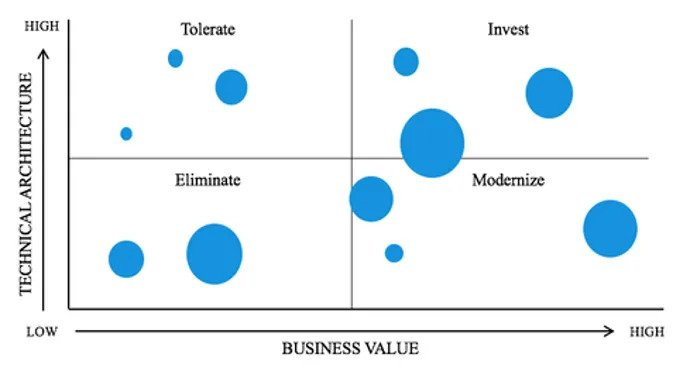
\includegraphics[width=12cm]{businessvalue}
\caption{Visuale representatie van businesswaarde voor mainframeapplicaties \autocite{Marble2017}}
\end{figure}



\subsection{\IfLanguageName{dutch}{Workloads migreren naar de cloud - Microservices}{Migrating workloads to the cloud - Microservices}}
\label{sec:Workloads migreren naar de cloud}

Een service is het ophalen of publiceren van data aan een remote systeem \autocite{Linthicum2016}. Volgens \textcite{Linthicum2016} is een voorbeeld hiervan het proces om een risicoanalyse te berekenen bij een financiële transactie. Dat is de fundamentele werking achter een service-oriented architecture (SOA). Microservices is daarnaast ook een architectuur, maar wordt volgens \textcite{Linthicum2016} vaak verward met een service-oriented architecture (SOA). Er is natuurlijk wel een bepaalde overlap in de twee technologieën. Het ontwerppatroon dat erachter zit, werkt door applicaties die bestaan uit kleine processen die met elkaar communiceren door het gebruik van application programming interfaces (API). De bedoeling bij service-oriented computing is dat applicaties worden gereduceerd tot enkel het functionele om vervolgens een set aan te bieden van services aan andere applicaties of de applicatie zelf. Het idee hierachter is het hergebruiken van functionaliteit \autocite{Linthicum2016}. 

Het gebruik van containers speelt bij microservices een grote rol. Met containers is het mogelijk om bestaande applicaties te bundelen en de complexiteit te verlagen. Containers zorgen ervoor dat de applicaties niet meer afhankelijk zijn van hun onderliggende infrastructuurservices. Hierdoor is het mogelijk de toegang tot de opslag en resources los te koppelen van de applicaties en maakt dat de applicaties minder statisch \autocite{Linthicum2016a}. Microservices zijn net zo onafhankelijk en losgekoppeld. Het zijn geïsoleerde componenten die individueel kunnen gebruikt worden zonder effect op andere componenten. Het gebruik van Linux en/of Docker containers verzekeren dat services in dezelfde omgeving kunnen draaien  \autocite{Bucchiarone2018}.

Volgens het rapport van \textcite{Bucchiarone2018}, waarin zij de ervaring beschrijven van een migratie van een monolithisch systeem zoals mainframe naar Microservices, zal de mainframe voor lange tijd nog verbonden zijn aan de Microservice-technologie. Het zal mogelijk zijn om uiteindelijk de functionaliteiten van de mainframe te implementeren als nieuwe services. Dat zal bijgevolg resulteren in het definitief ontkoppelen van de mainframe \autocite{Bucchiarone2018}. 


\subsection{\IfLanguageName{dutch}{Workloads migreren naar de cloud - Amazon Web Services (AWS)}{Migrating workloads to the cloud - Amazon Web Services (AWS)}}
\label{sec:Workloads migreren naar de cloud}

Amazon Web Services (AWS) is een cloudplatform van Amazon. AWS biedt organisaties middelen als rekenkracht, databankopslag en informatieleveringsdiensten. Het cloudplatform van Amazon is gelanceerd in 2006 en is gebaseerd op de infrastructuur waar Amazon.com op draait. Daarnaast zijn zij de eerste die het pay-as-you-go cloud computing model aanbieden. Dat wil zeggen dat de infrastructuur geschaald wordt aan de hand van de opslag en noden van de klant op vlak van rekenkracht \autocite{Gillis2020}.

\subsubsection{\IfLanguageName{dutch}{AWS Mainframe Modernization Service}{AWS Mainframe Modernization Service}}
\label{sec:AWS Mainframe Modernization Service }

In december 2021 vond een event plaats waar de AWS Mainframe Modernization Service is geïntroduceerd. De spreker van dat event was de principal product manager van AWS, genaamd de Valence. Volgens hem staan veel bedrijven voor grote uitdagingen wat hun mainframeplatform betreft. Veel organisaties komen met de vraag hoe zij hun assets van op hun mainframearchitectuur kunnen migreren naar AWS \autocite{Valence2021}. Hij kaart volgende problemen met het mainframeplatform aan: 
 \begin{itemize}
    \item Complexe afhankelijkheden
    \item Beperkte en trage innovatie
    \item Oplopende kosten
    \item Gebrek aan skills
    \item Ontoegankelijke data
    \item Strikte afhankelijkheden
    \item Gelimiteerde capaciteit
    \item Outdated interfaces 
    \item Legacy componenten
    \item Ongedocumenteerde applicaties 
    \item Langdurige investering 
\end{itemize}

De voornaamste redenen volgens \textcite{Valence2021} die bedrijven die willen migreren aankaarten, zijn om hun kosten te reduceren, risico's te verminderen en hun flexibiliteit te verhogen. Met flexibiliteit bedoelt hij dat organisaties zo snel mogelijk kunnen beantwoorden aan externe veranderingen zoals de vraag van de klant of de hoeveelheid dataverwerking. Daarnaast willen organisaties de kosten die de mainframe met zich meebrengt omruilen voor investeringen in nieuwe innovaties. Deze vereisten zijn de dreefveer achter de migratieplannen, maar willen zij tegelijk de RAS-factoren (reliabilty, availability, serviceability) die de mainframe biedt behouden bij een migratie naar een cloudomgeving. AWS Mainframe Modernization Service is volgens \textcite{Valence2021} een uniek platform voor het migreren, moderniseren en uitvoeren van mainframeapplicaties. Deze service is in staat om mainframeapplicaties uit te voeren en te beheren. Bij het migreren naar het AWS-platform zijn vier fases betrokken, waaronder analyseren, ontwikkelen, deployen en beheren. Zoals aangegeven bij vorige strategieën, waaronder die van \textcite{Marble2017}, is analyseren van de workloads een belangrijk onderdeel. Het is belangrijk om een kijk te nemen naar alle afhankelijkheden, businesswaarde en complexiteit van elke applicatie om te kunnen bepalen in welke volgorde de migratie wordt uitgevoerd. 

De tweede fase is de ontwikkelfase. Dat is de fase waar de migratie gebeurt, zoals het hercompileren, herformatteren van data of conversies om te voldoen aan de artefacten van de nieuwe doelapplicatie. Bij de deployfase vertelt \textcite{Valence2021} dat hier de unieke mogelijkheden verborgen zitten van de AWS Mainframe Modernization Service. Hier wordt namelijk een runtime omgeving opgezet voor de mainframeapplicaties. De bedoeling is dat een organisatie een runtime omgeving volledig zelf kan creëren en hun applicaties hierop bijgevolg kunnen deployen. 

Via AWS Blu Age is het mogelijk om aan automatische code refactoring te doen. Hierbij is het mogelijk gemaakt om legacy applicaties, die werden geschreven in COBOL of PL/1, te refacteren naar Java of batchscripts. De AWS Blu Age is een ketting van verschillende stappen binnen het moderniseren. Er zal aan reverse-engineering en forward-engineering gedaan worden om runtime instanties te kunnen verkrijgen van applicaties geschreven in een mainframespecifieke programmeertaal. Volgens \textcite{Valence2021} is de bedoeling van de AWS Blu Age Toolchain om een moderne Angular front-end webservice te krijgen die Java services aanspreekt via een REST API op basis van de mainframe legacy.  

Bij het opzetten van een moderniseringsproject voor het migreren van mainframe naar AWS, volgt AWS een plan dat gebaseerd is op het Migration Accelaration Program (MAP). Dat programma is afkomstig van gedistribueerde systemen en is een waardig cloudmigratieprogramma. Het is gebaseerd op duizenden best practices op vlak van een migratie. AWS heeft dat programma aangepast zodat het specifiek inzetbaar is voor een migratie van een mainframeplatform. Volgens \textcite{Valence2021} geeft het programma een garantie op het slagen van migratieprojecten. Het MAP steunt op zes pilaren waaronder:
 \begin{itemize}
    \item Migratiemethodologieën
    \item AWS tools
    \item AWS partners
    \item AWS investeringen
    \item AWS trainingen
    \item AWS professionele services
\end{itemize}

AWS raadt sterk aan om bij een migratieproject, dat gebruik maakt van de AWS Mainframe Modernization Service, een expert of meerdere experten aan te werven die kennis hebben van de toolchains die AWS aanbiedt. Volgens \textcite{Valence2021} is het van essentieel belang dat organisaties hulp inroepen van specialisten om het succes van een migratieproject te garanderen. 

\subsubsection{\IfLanguageName{dutch}{Een praktische uitwerking: het uitvoeren van een COBOL applicatie op AWS Lambda}{A practical implementation: running a COBOL application on AWS Lambda}}
\label{sec: Een praktische uitwerking: uitvoeren  van COBOL applicatie op AWS Lambda}

Met deze praktische uitwerking wordt aangetoond hoe eenvoudig of complex het is om  gebruik te maken van de functies die AWS aanbiedt om aan migratie te doen.

Via AWS Lambda is het mogelijk om via hosted services aan serverless computing te doen op AWS. Volgens \textcite{Sbarski2017} is serverless computing een bevestiging van hoe een intelligente combinatie van services een vermindering kan teweegbrengen op vlak van de tijd en de kosten die ontwikkeling met zich meebrengt. Deze nieuwe architectuur laat de kosten die serversoftware of mainframesoftware met zich meebrengen verdwijnen. Daarnaast biedt het de flexibiliteit om snel te ontwikkelen, deployen en applicaties te beheren \autocite{Sbarski2017}. Lambda kan code uitvoeren op een extreem parallelle manier als respons op een event. Zonder behulp van servers is het mogelijk om via Lambda code uit te voeren. Het is niet meer nodig om na te denken over het installeren van software, het deployen van containers of andere details \autocite{Sbarski2017}. AWS zorgt ervoor dat hun Elastic Compute Cloud (EC2) servers de code uitvoert met in het achterhoofd zaken te voorzien als schaalbaarheid en beschikbaarheid. Zodat de ontwikkelaar hier niet meer over hoeft na te denken. Serverless architectuur verwijst naar een architectuur waar het niet meer noodzakelijk is om een directe connectie te hebben met een mainframe of server. Als gevolg hiervan moeten ontwikkelaars zich enkel focussen op het kwalitatief schrijven van code. Hieronder bevinden zich de vijf principes waar een serverless architectuur op steunt:
 \begin{itemize}
    \item Het gebruik van een compute service om code uit te voeren zonder servers of mainframes
    \item Het schrijven van functies met één enkel doel
    \item Event-driven pipelines
    \item Het bouwen van krachtigere front-ends
    \item Het gebruik van third-party services
\end{itemize}

AWS Lambda is een compute service die code uitvoert op de Amazon Web Services infrastructuur. De broncode van applicaties wordt uitgepakt en gedeployed op een geïsoleerde container met zijn eigen gealloceerd geheugen en central processing unit. De combinatie van code, configuraties en afhankelijkheden staan bekend onder een Lambda functie. Lambda ondersteunt daarnaast push en pull events en integreert een groot aantal AWS services. 
\begin{figure}[h]
    \centering
    \begin{subfigure}{0.45\textwidth}
        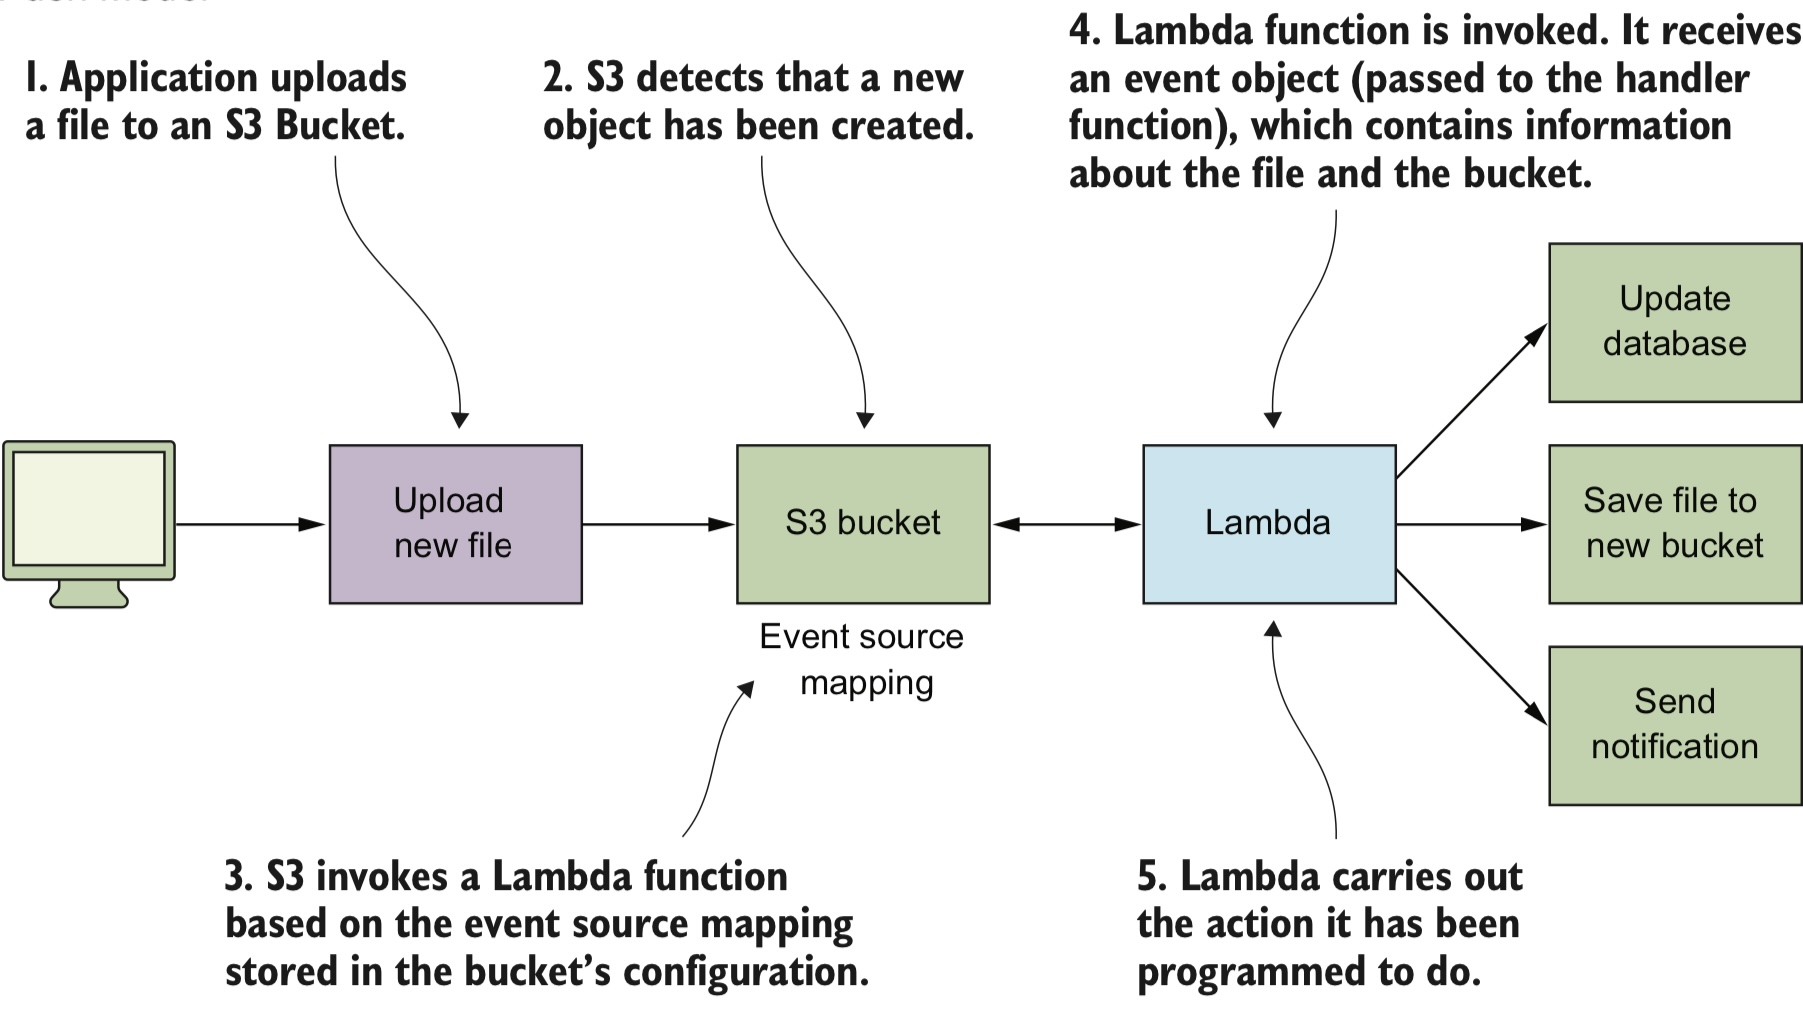
\includegraphics[width=\textwidth]{push_model}
        \caption{Voorbeeld van het push model \autocite{Sbarski2017}}
    \end{subfigure}
    \hfill
    \begin{subfigure}{0.45\textwidth}
        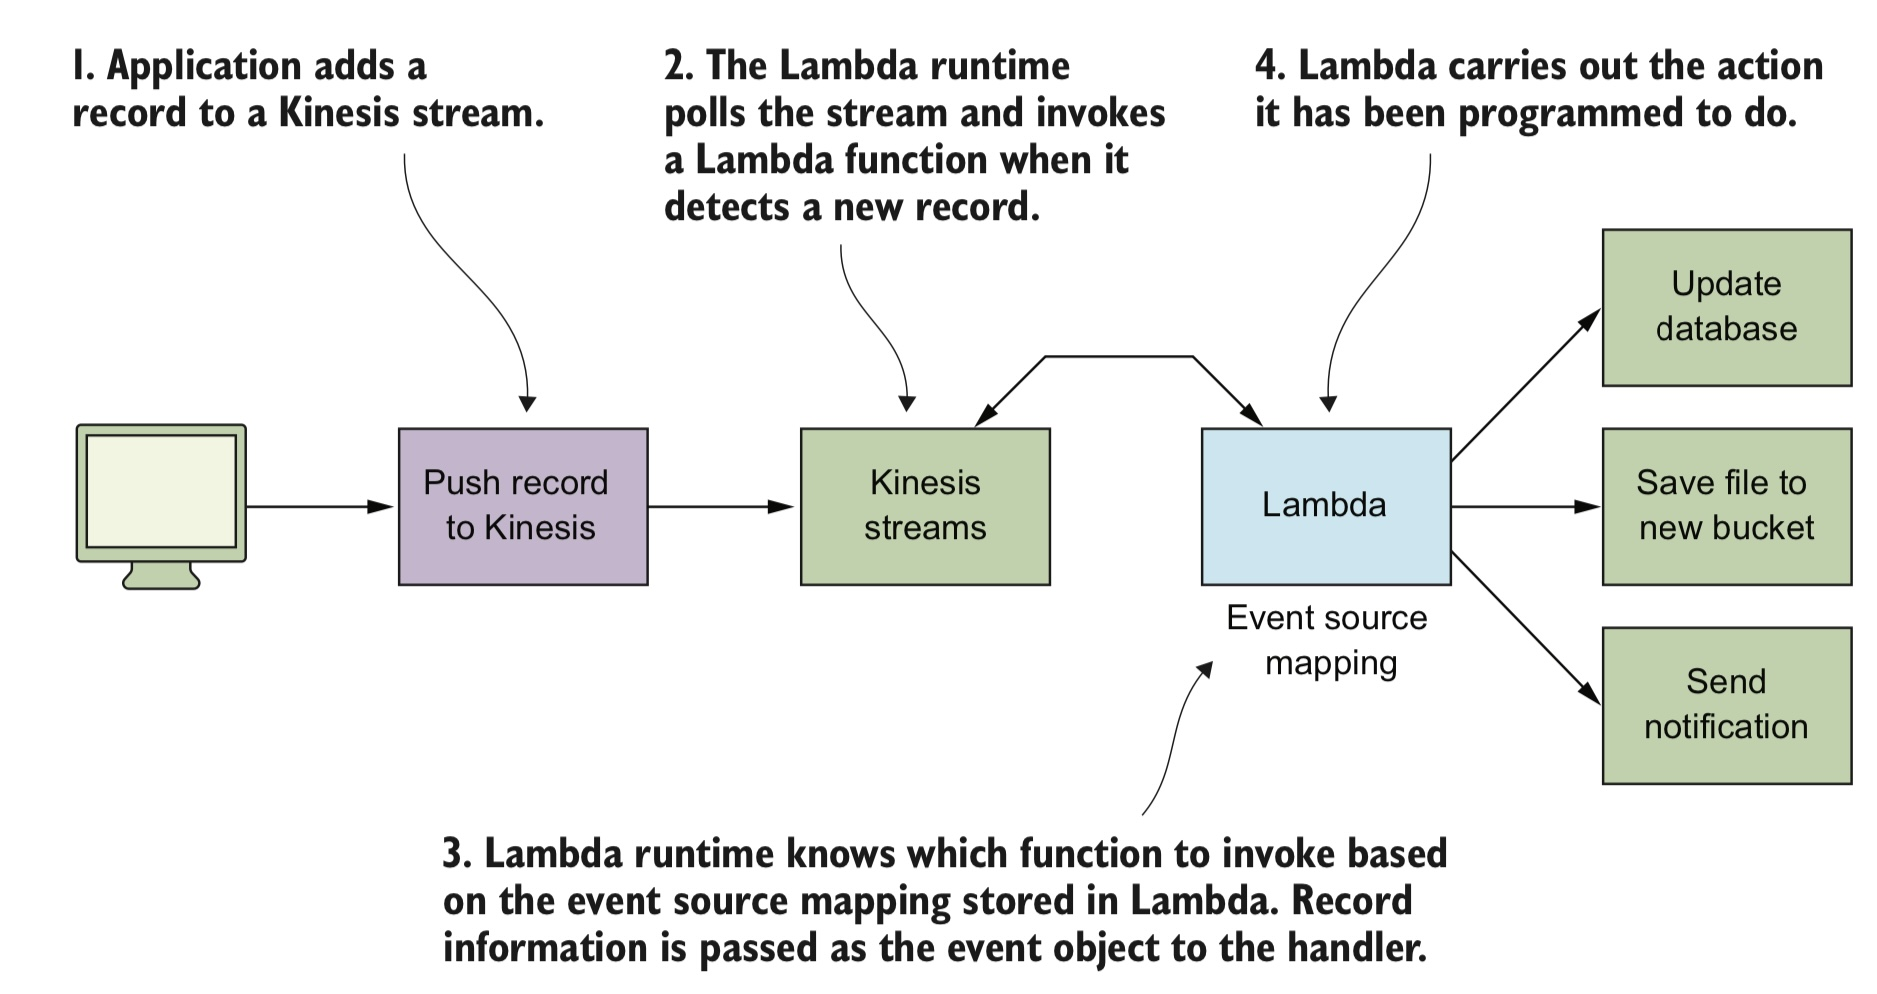
\includegraphics[width=\textwidth]{pull_model}
        \caption{Voorbeeld van het pull model \autocite{Sbarski2017}}
    \end{subfigure}
\end{figure}

\newpage

Als praktische uitwerking is in dit onderzoek met behulp van een AWS Lambda functie een kleine COBOL-applicatie gedeployed op het AWS-platform. Deze uitwerking werd gedaan met behulp van het stappenplan van \textcite{Paika2020}. Volgens \textcite{Paika2020} is dat een ideale manier om aan te tonen hoe een AWS Lambda functie in zijn werk gaat. Eerst en vooral moet de COBOL-code voor een simpel 'Hello World ' programma lokaal gecompileerd en uitgevoerd worden in een terminal zoals hieronder weergegeven. De compiler die in het onderzoek werd gebruikt is GnuCOBOL.  
    \begin{figure}[h]
        \centering
        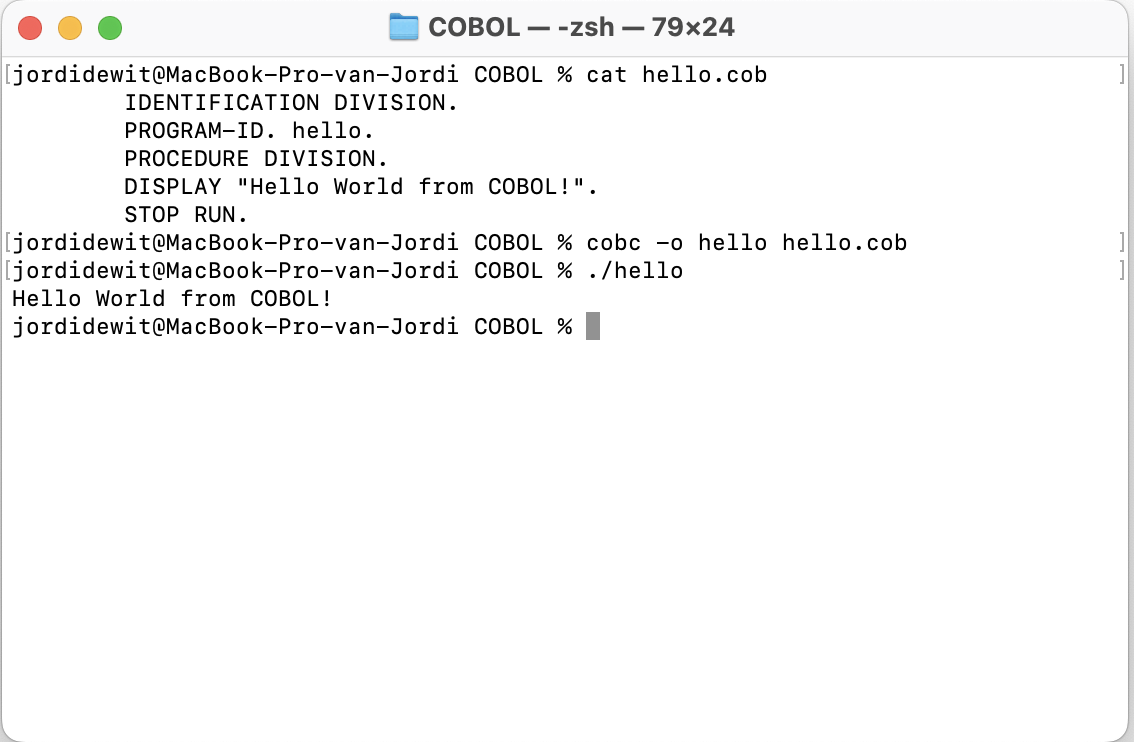
\includegraphics[width=7cm]{gnucobol}
        \caption{Het lokaal uitvoeren van een COBOL programma met GnuCOBOL.}
     \end{figure}
 
 \newpage
 
 Volgens het stappenplan van \textcite{Paika2020} is het de bedoeling dat er een runtimeomgeving wordt opgezet door gebruik te maken van een AWS Lambda functie. Dat kan bereikt worden via de Amazon Linux 2 AWS Lambda executieomgeving. Hiervoor is het nodig om een bootstrap script te creëren om een uitvoering te voorzien zodra de Lambda functie wordt geïnitialiseerd. Amazon Linux 2 kan worden gevirtualiseerd in een docker file. Hier is het mogelijk om het COBOL-programma te compileren omdat Amazon Linux 2 ook gebruik maakt van de  GnuCOBOL-compiler. 
 
 Er moet vervolgens een docker file aangemaakt worden. Hiervoor is het mogelijk om de texteditor Vim te gebruiken. Het bestand met de instructies in voor het aanmaken van de docker image, dient zich in een lege directory te bevinden samen met het bestand waar de code van de COBOL-applicatie instaat. Deze stappen werden niet uitgelegd in de gids van \textcite{Paika2020}. Deze zijn echter van essentieel belang voor het slagen van het project. Op onderstaande afbeelding is te zien hoe dat proces in zijn werk ging. 
 
  \begin{figure}[h]
     \centering
     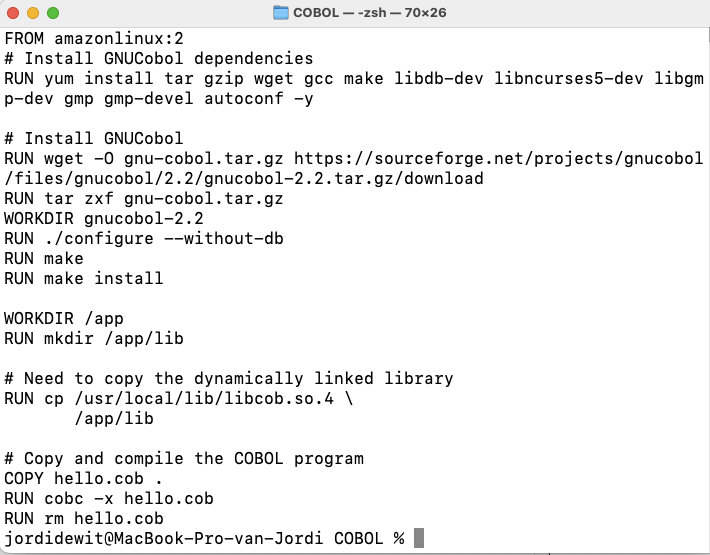
\includegraphics[width=7cm]{bootstrap_script}
     \caption{De docker file met instructies voor de docker image aan te maken.}
 \end{figure}

  \begin{figure}[h]
    \centering
    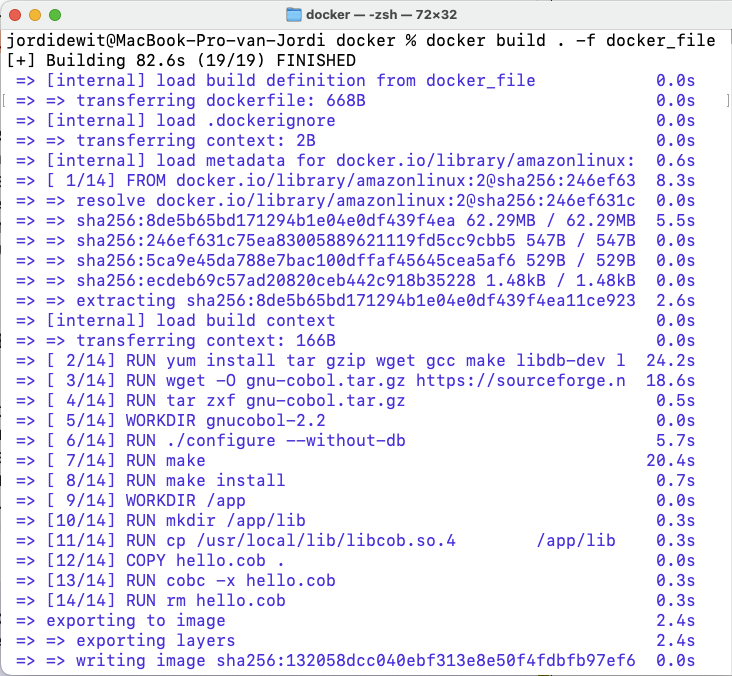
\includegraphics[width=7cm]{build_imag}
    \caption{De uitvoering van het bootstrap script voor het aanmaken van de docker image.}
\end{figure}

\newpage
Het onderstaande script build.sh zorgt ervoor dat een uitvoerbaar bestand wordt gekopieerd vanuit de docker container naar het lokale bestandssysteem. Dat bestand dient voor het deployen naar Amazon Web Services. 

  \begin{figure}[h]
    \centering
    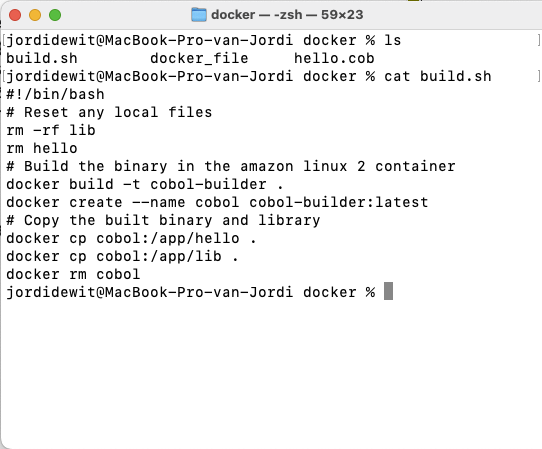
\includegraphics[width=7cm]{script}
    \caption{Het aanmaken van het build.sh bestand voor het kopiëren van het uitvoerbaar bestand.}
\end{figure}

Hieronder bevindt zich een afbeelding van het hello bestand dat is aangemaakt door build.sh. Dat bestand is mogelijk om uit te voeren in AWS Lambda.

  \begin{figure}[h]
    \centering
    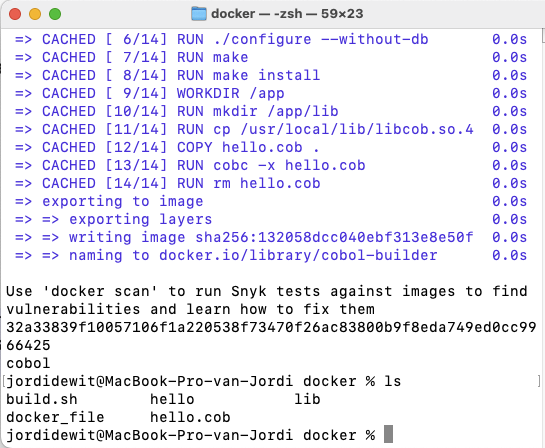
\includegraphics[width=7cm]{executable}
    \caption{Het uitvoerbaar bestand hello in de COBOL directory.}
\end{figure}

\newpage
In de volgende stap is het de bedoeling dat er een Lambda runtimeomgeving wordt opgezet. Hiervoor dient opnieuw een bootstrap script geschreven te worden die verantwoordelijk is voor het bootstrappen van de runtime-omgeving. Het volgende script is opgesteld aan de hand van een tutorial die AWS aanbiedt \autocite{AWS2022}. 

 \begin{figure}[h]
    \centering
    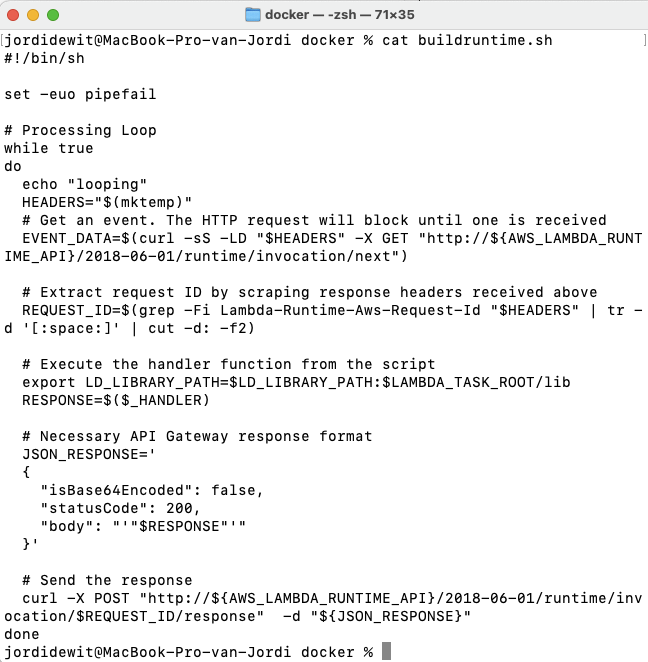
\includegraphics[width=7cm]{buildruntime}
    \caption{Het runtimeomgevingsscript volgens de tutorial van \autocite{AWS2022}.}
\end{figure}

In de laatste stap naar een succesvol deployment van de COBOL-applicatie moet de Lambda functie en de API Gateway gecreëerd worden. Wat in een eerdere paragraaf werd aangekaart, is het serverless computing principe. Om dat principe toe te passen dient er eerst een package ``serverless `` geïnstalleerd te worden voor het serverless.yaml bestand te kunnen aanmaken dat onze Lambda functie en API Gateway definieert. 

 \begin{figure}[h]
    \centering
    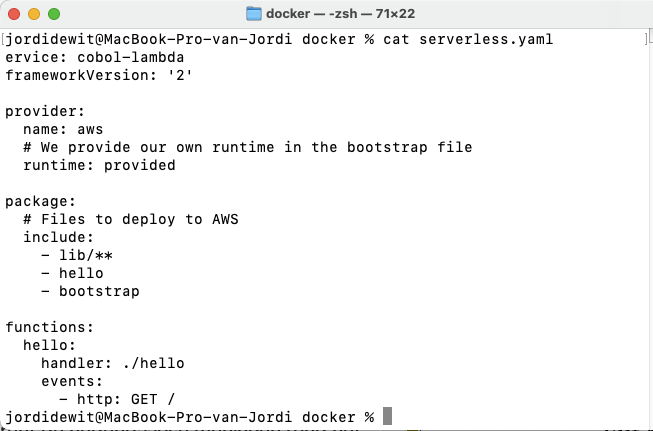
\includegraphics[width=7cm]{serverless}
    \caption{Het serverless.yaml bestand voor het defniëren van de Lambda functie en API Gateway.}
\end{figure}

\newpage

Het bovenstaande script zorgt ervoor dat ons programma hello gedefinieerd is als functie. Wanneer deze opgeroepen wordt zal er een HTTP GET request gemaakt worden naar de API Gateway. Hierbij kwam een einde aan alle stappen die \textcite{Paika2020} uitgewerkt heeft. Bij het uitvoeren van het script build.sh is het COBOL-programma gedeployed op AWS Lambda en zichtbaar in de browser. De migratie is compleet.

 
 \section{\IfLanguageName{dutch}{De resultaten van de bevragingen}{The results of the survey}}
 \label{sec:De resultaten van de bevraging}
 
 Om in dit onderzoek ook een beeld te kunnen schetsen omtrent de hedendaagse meningen rond het gebrek aan expertise, migratieplannen en interesse voor mainframe bij studenten en IT-professionals werd een enquête opgesteld. Deze enquête heeft volgende resultaten opgeleverd.
 
  \subsection{\IfLanguageName{dutch}{De resultaten van de bevragingen voor bedrijven}{The results of the survey for organizations}}
 \label{sec:De resultaten van de bevraging}

Vijf bedrijven hebben geantwoord op de enquête. Volgende bedrijven namen deel: 
 \begin{itemize}
    \item KBC
    \item Colruyt Group
    \item Nationaal Vebond van Socialistische Mutualiteiten
    \item SD Worx
    \item Volvo Group
\end{itemize}

Verder zijn de resultaten te vinden die opgedeeld zijn per vraag. 

 \subsubsection{\IfLanguageName{dutch}{In welke sector is het bedrijf actief?}{In which sector is the organization active?}}
\label{sec:In welke sector is het bedrijf actief}

 \begin{figure}[h]
    \centering
    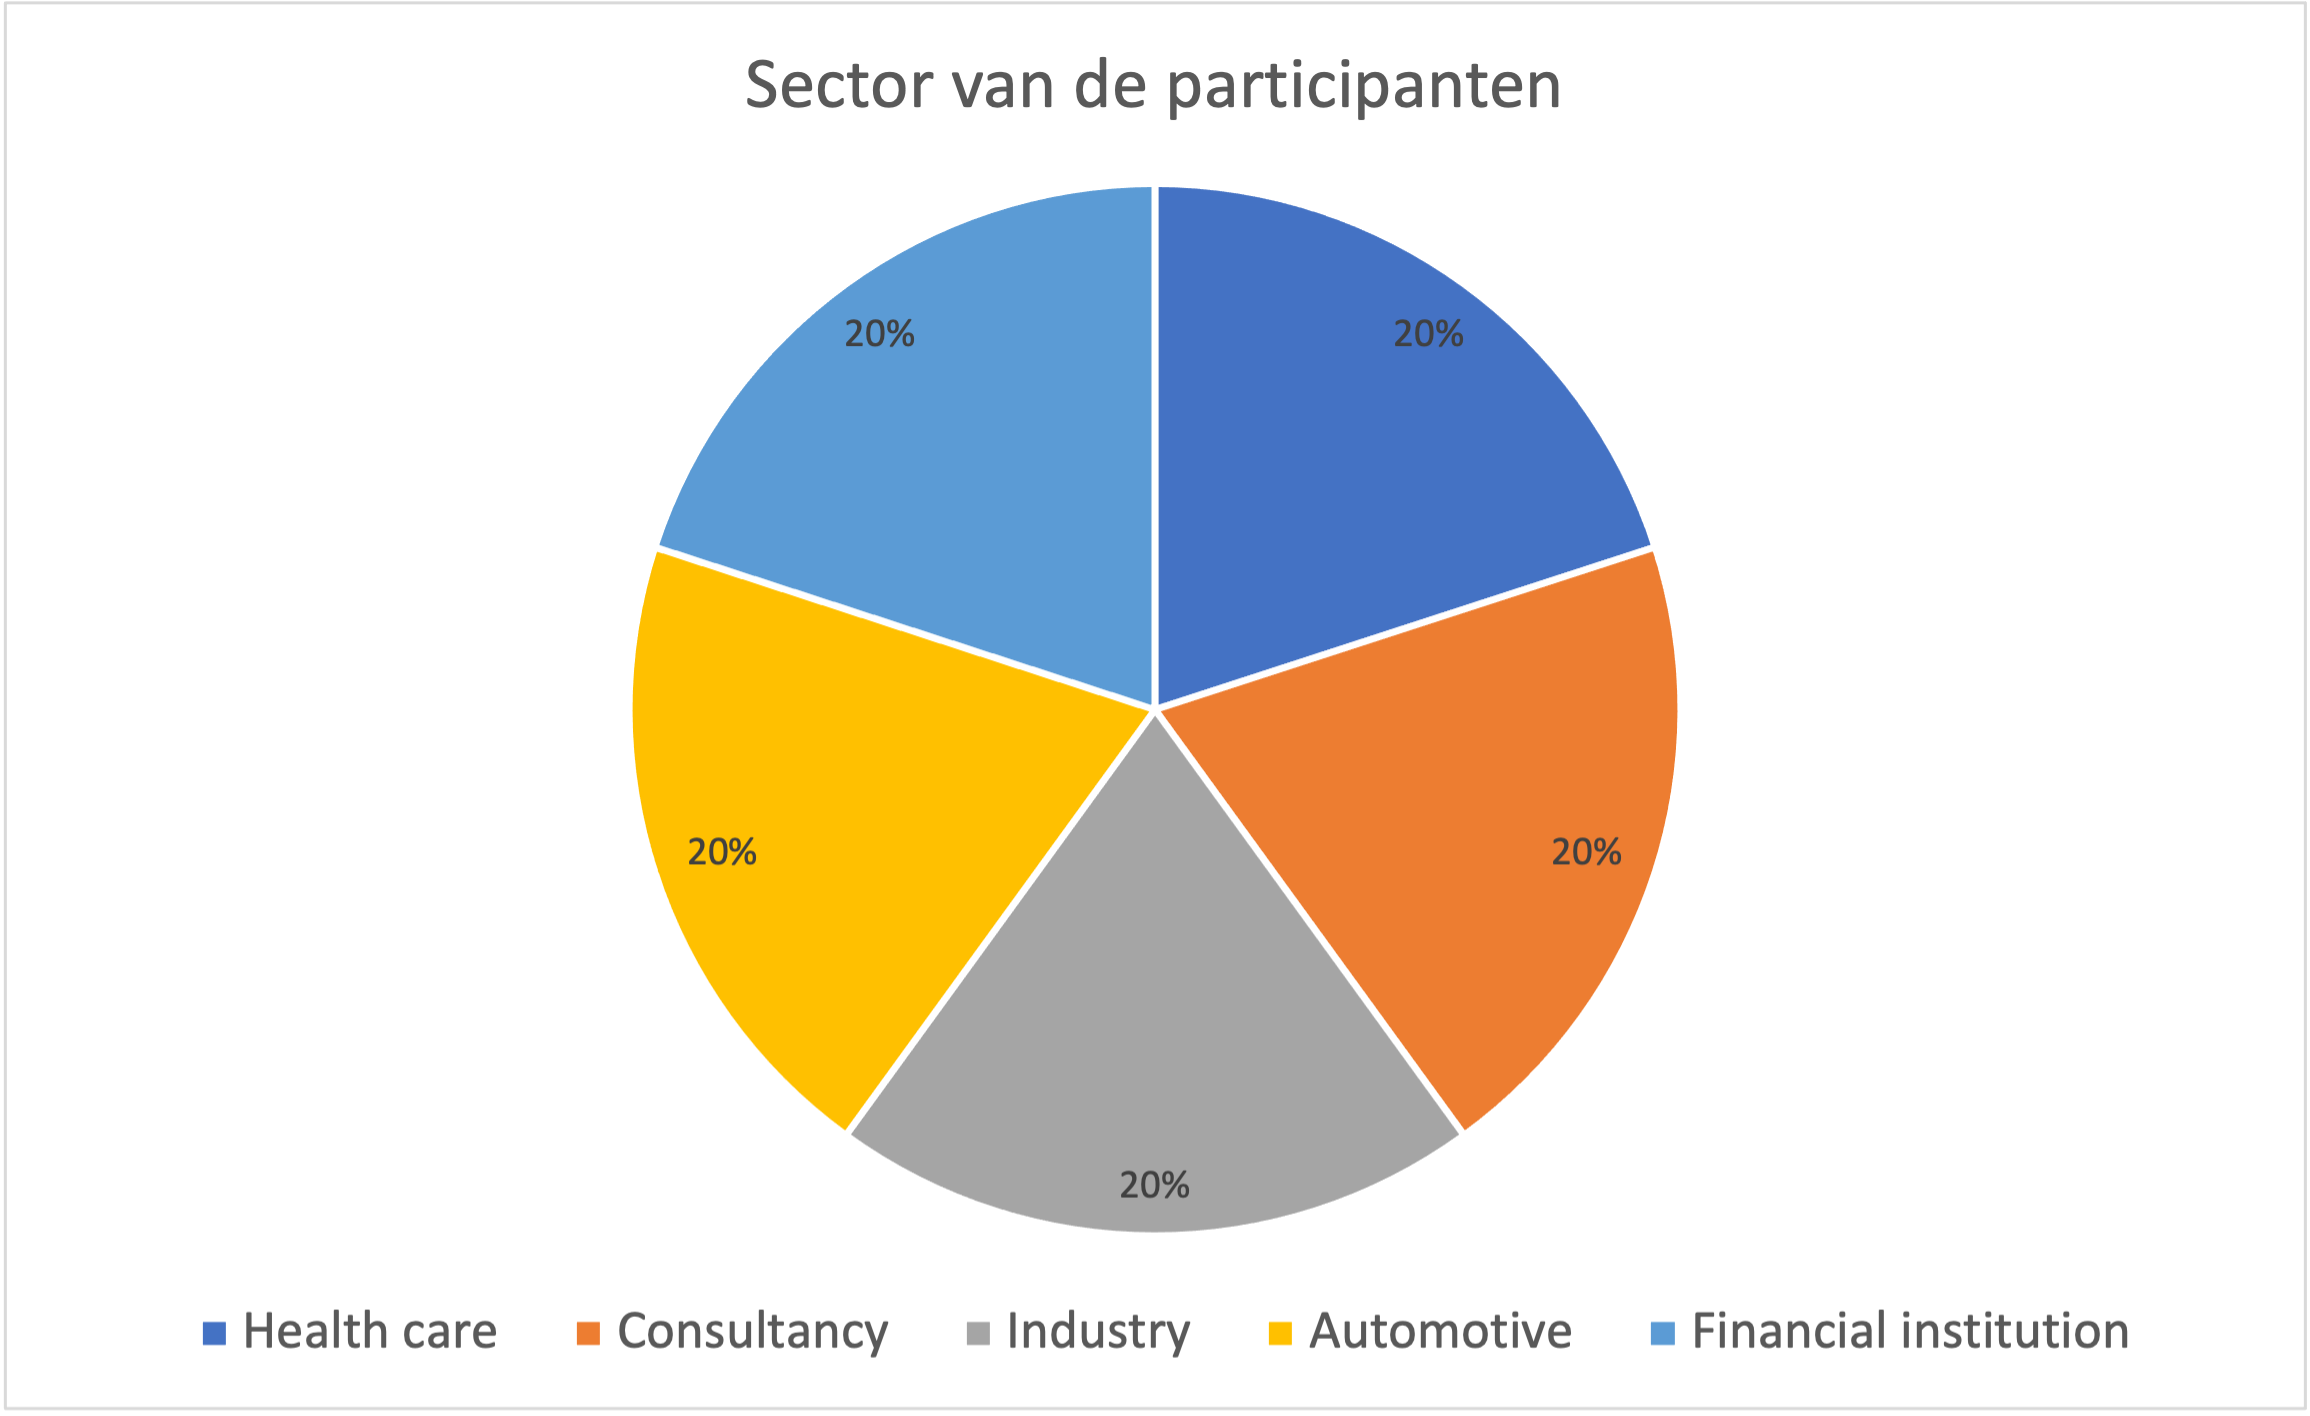
\includegraphics[width=10cm]{sector_grafiek}
    \caption{De verdeling van de deelnemende organisaties per sector.}
\end{figure}

Uit bovenstaande grafiek is af te leiden dat de participanten die geclassificieerd worden als een bedrijf gelijk verdeeld zijn. Uit elke sector heeft telkens één bedrijf deelgenomen aan de bevraging rond het onderzoek. Daarnaast heeft elk bedrijf een mainframe in gebruik. 


 \subsubsection{\IfLanguageName{dutch}{Wat is het aantal werknemers die werk leveren dat te maken heeft met het ontwikkelen, onderhouden of beheren van een mainframe?}{What is the number of employees who develop, maintain or manage a mainframe?}}
\label{sec:Wat is het aantal van werknemers die werk leveren dat te maken heeft met het ontwikkelen, onderhouden of beheren van een mainframe?}

 \begin{figure}[h]
    \centering
    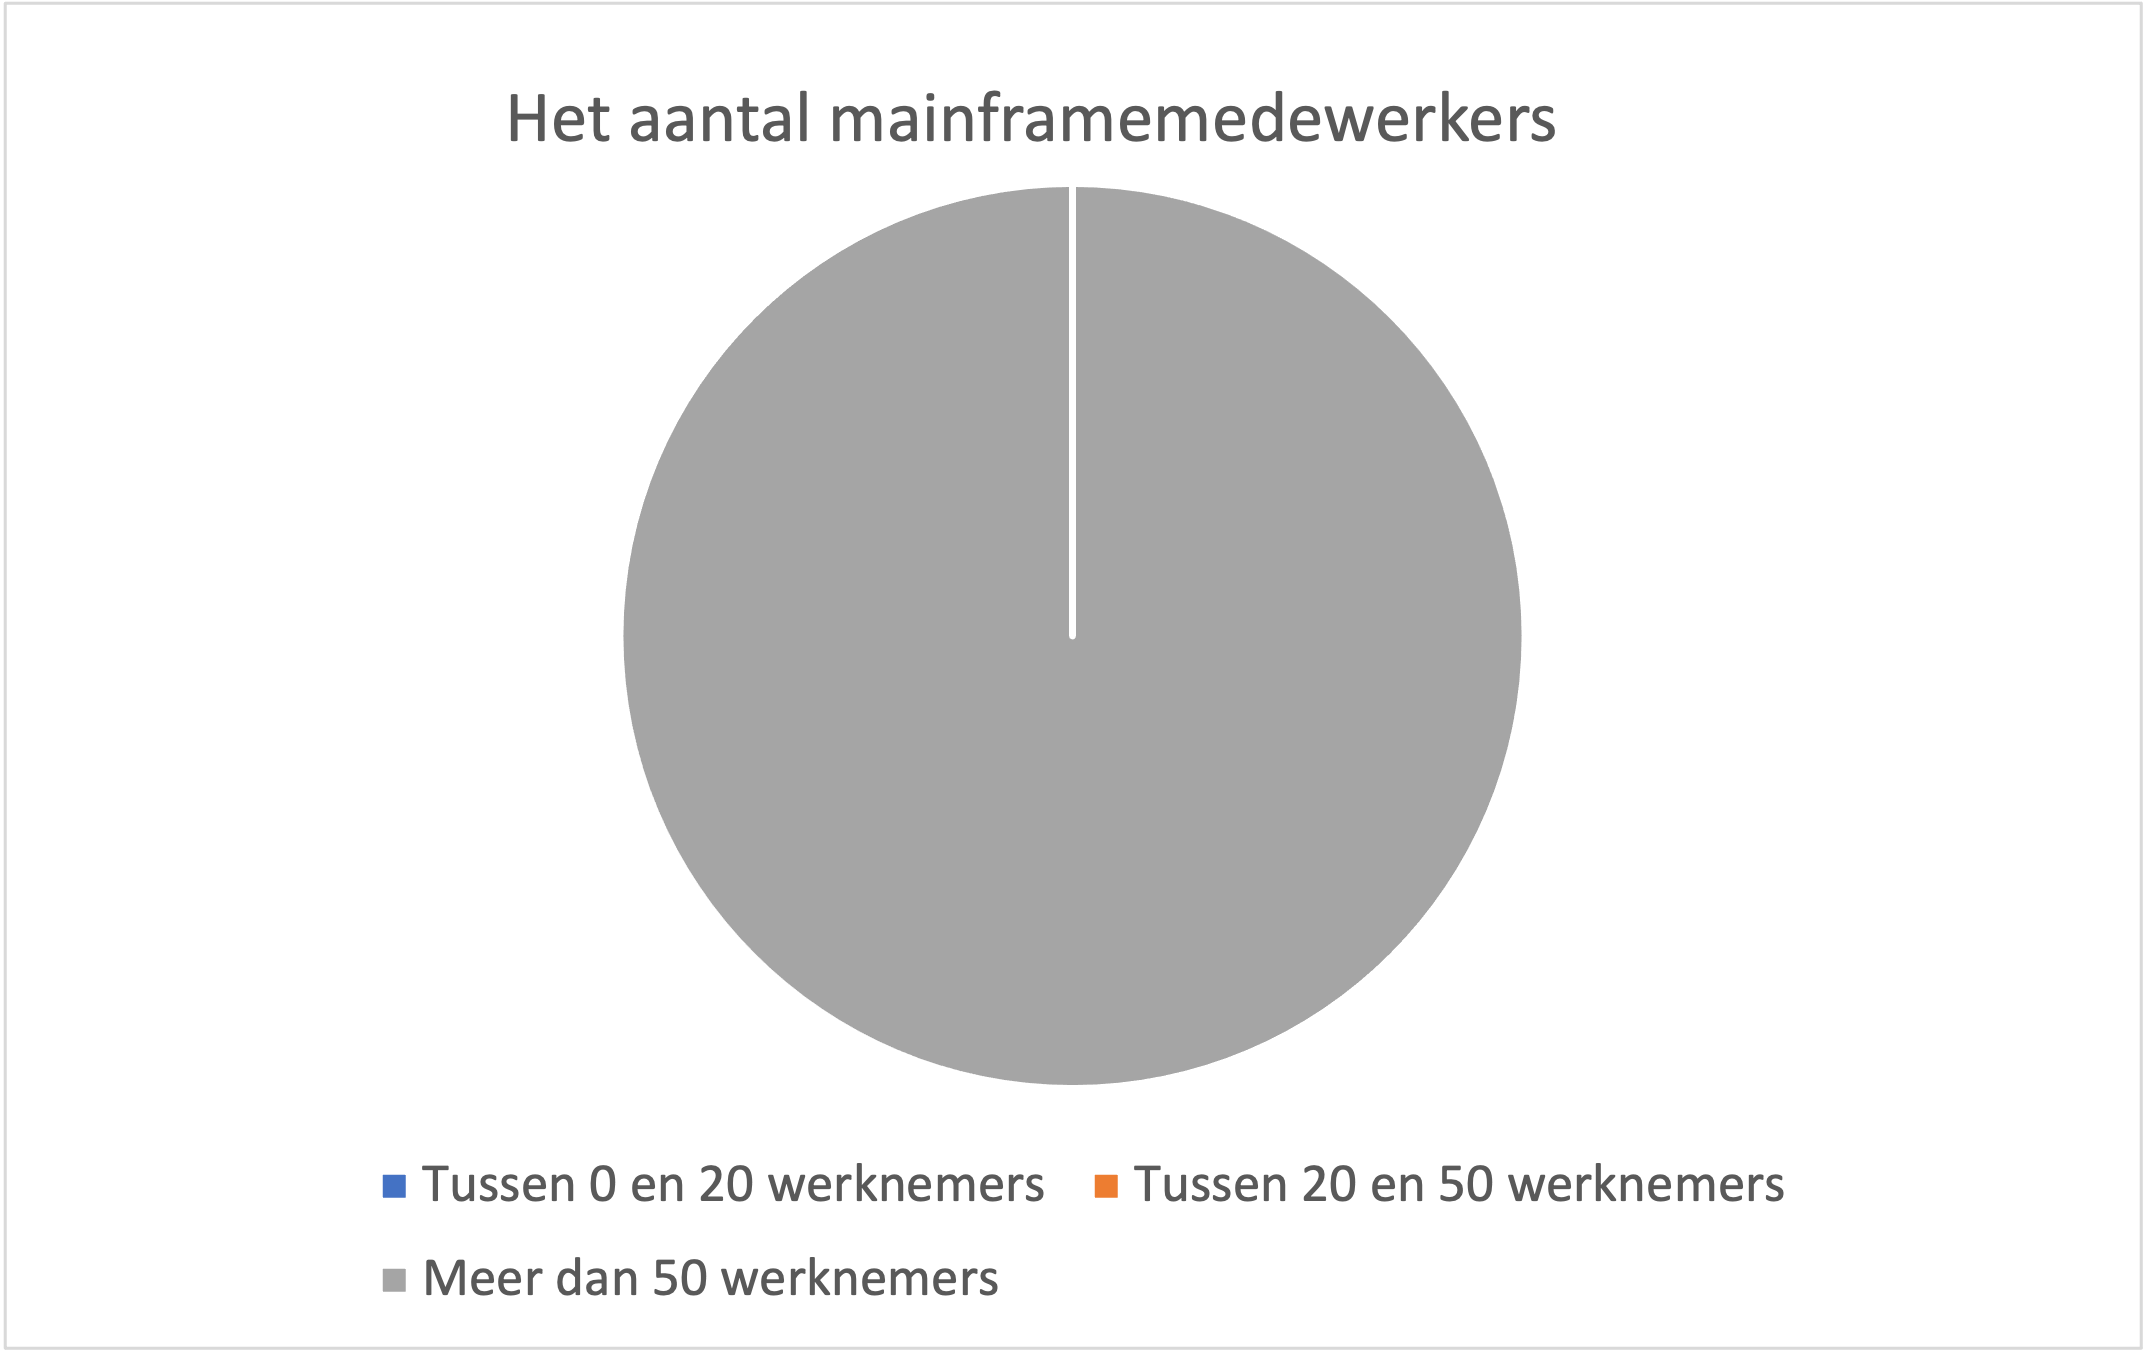
\includegraphics[width=10cm]{werknemers_grafiek}
    \caption{De grafiek met het aantal werknemers dat op mainframe werkt.}
\end{figure}

Elk van de bevraagde bedrijven heeft meer dan 50 mensen in dienst die werken op mainframe. Dat omvat het ontwikkelen, het onderhouden van applicaties of beheren van het systeem. Hieruit kan geconcludeerd worden hoe hoog de nood is aan mainframewerkkrachten. Deze werkkrachten zijn namelijk een groot deel van een IT-afdeling binnen de deelnemende organisaties.

\newpage

 \subsubsection{\IfLanguageName{dutch}{Wat is de gemiddelde leeftijd van het mainframepersoneel?}{What is the average age of the mainframe staff?}}
\label{sec:Wat is de gemiddelde leeftijd van het mainframepersoneel?}

\begin{figure}[h]
    \centering
    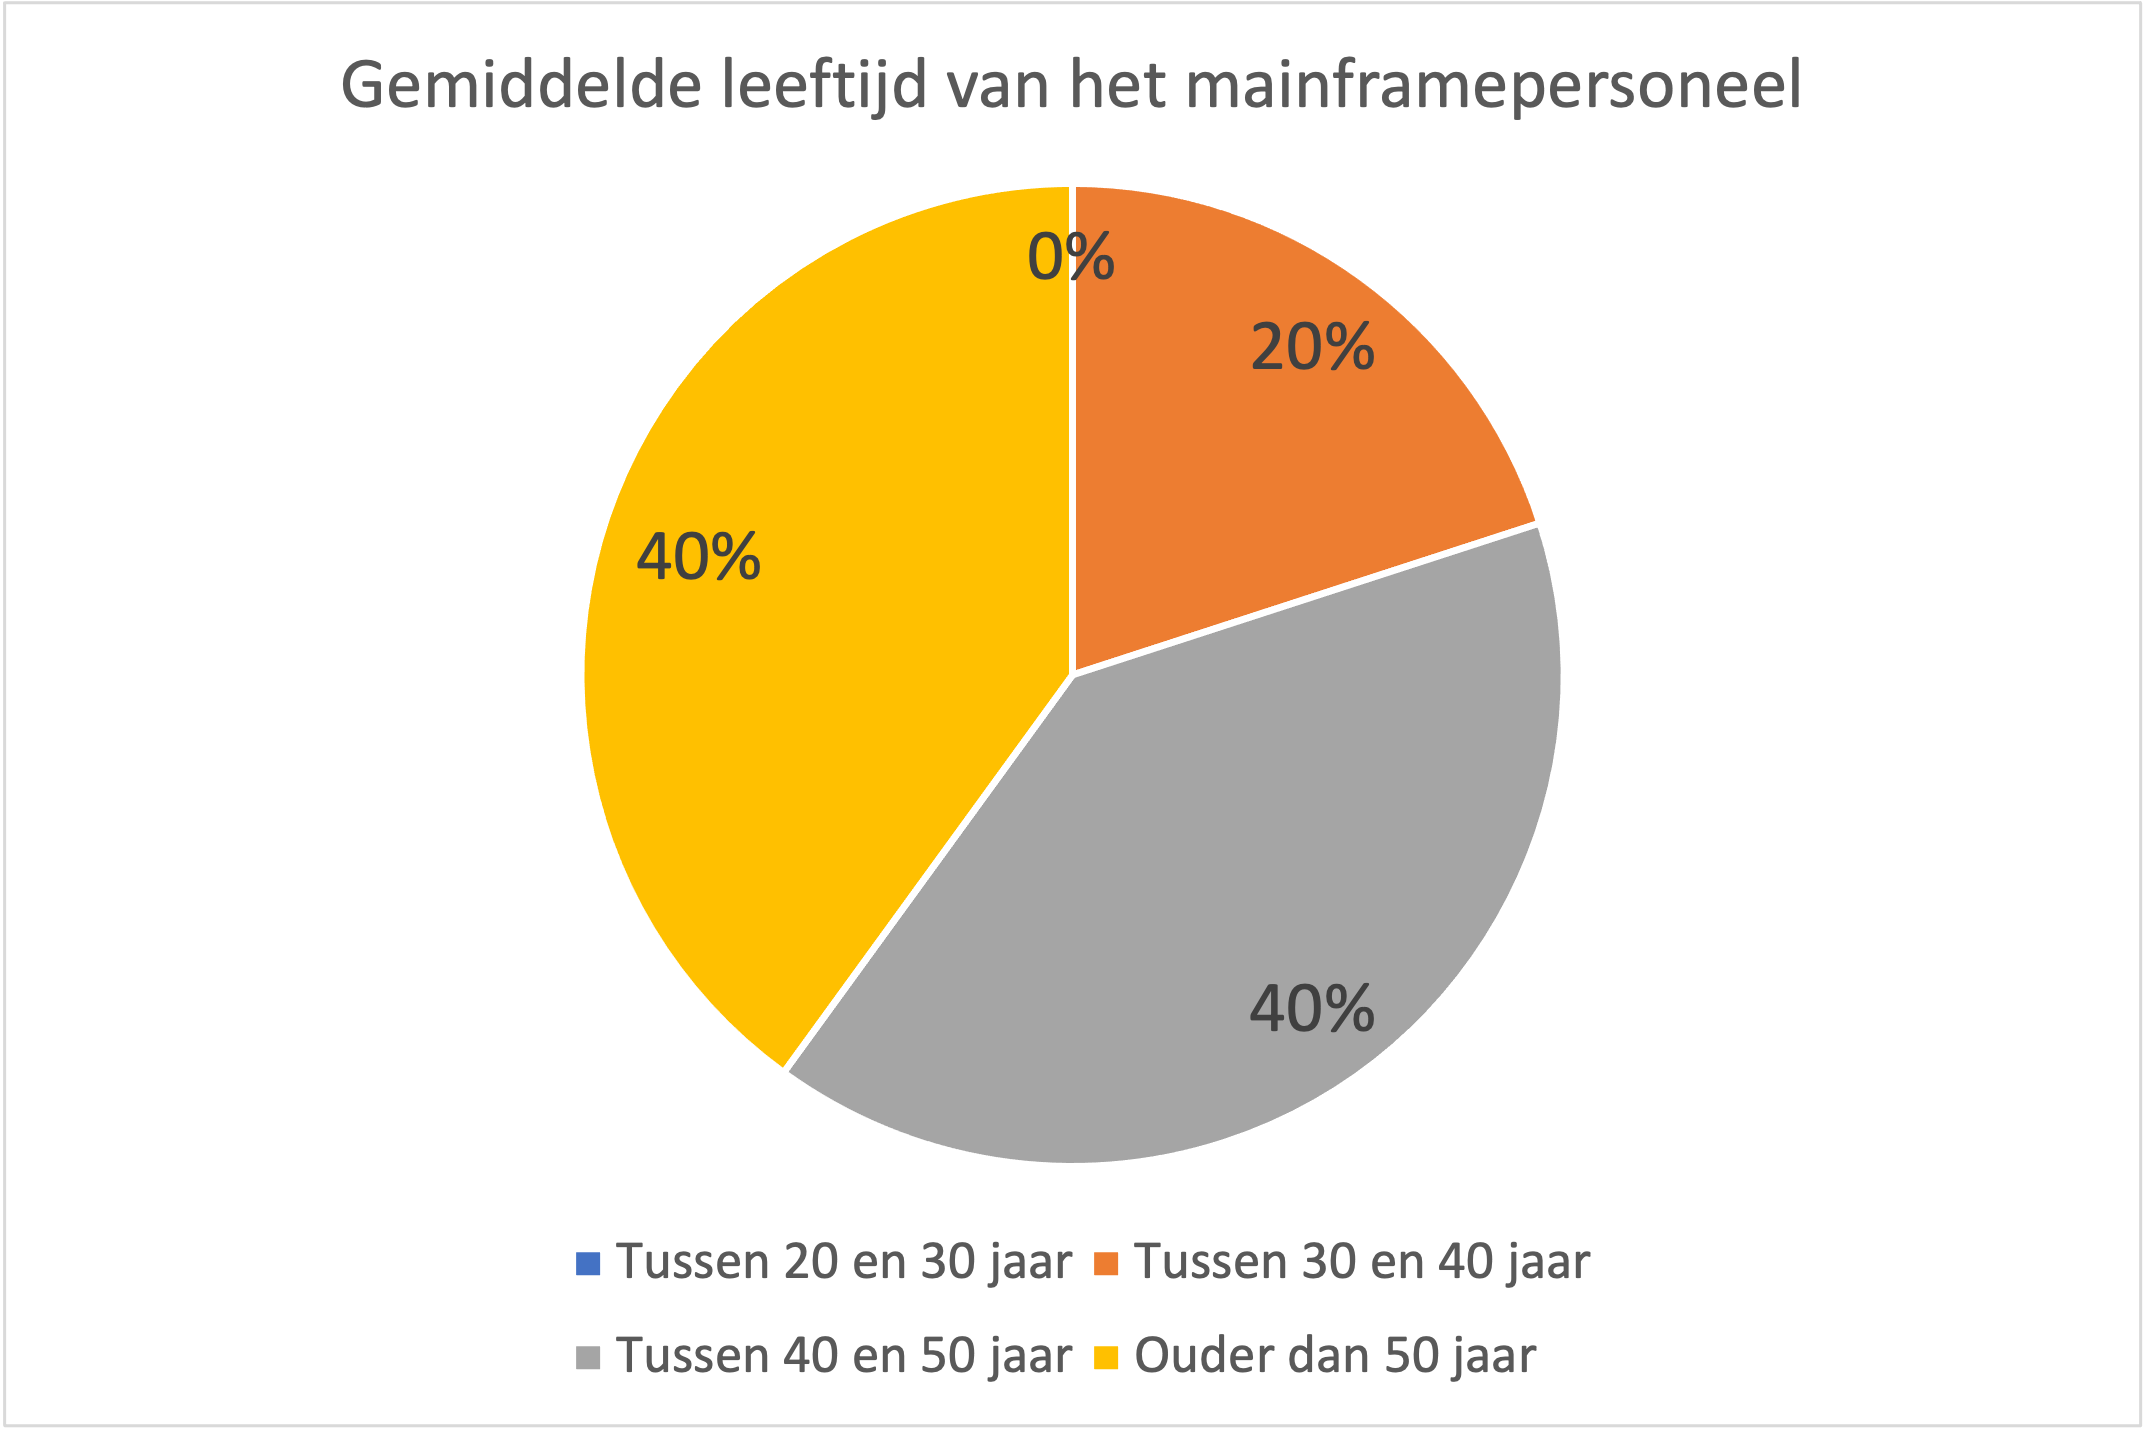
\includegraphics[width=10cm]{gemiddelde_leeftijd_grafiek}
    \caption{De grafiek met de gemiddelde leeftijd van het mainframepersoneel.}
\end{figure}


De gemiddelde leeftijd binnen de deelnemende organisaties ligt opmerkelijk hoog. Twee van vijf bedrijven geeft aan dat hun mainframepersoneel een gemiddelde leeftijd heeft die hoger ligt dan 50 jaar. Slechts één bedrijf geeft aan dat hun mainframepersoneel een gemiddelde leeftijd heeft tussen 30 en 40 jaar ligt. De andere bedrijven geven een leeftijd aan tussen 40 en 50 jaar. 

\newpage 

  \subsubsection{\IfLanguageName{dutch}{Zijn er signalen die aangeven of er een tekort is aan nieuwe mainframe-experten?}{Are there any signals that there is a shortage of new mainframe experts?}}
 \label{sec:Zijn er signalen die aangeven of er een tekort is aan nieuwe mainframe-experten?}
 
 \begin{figure}[h]
     \centering
     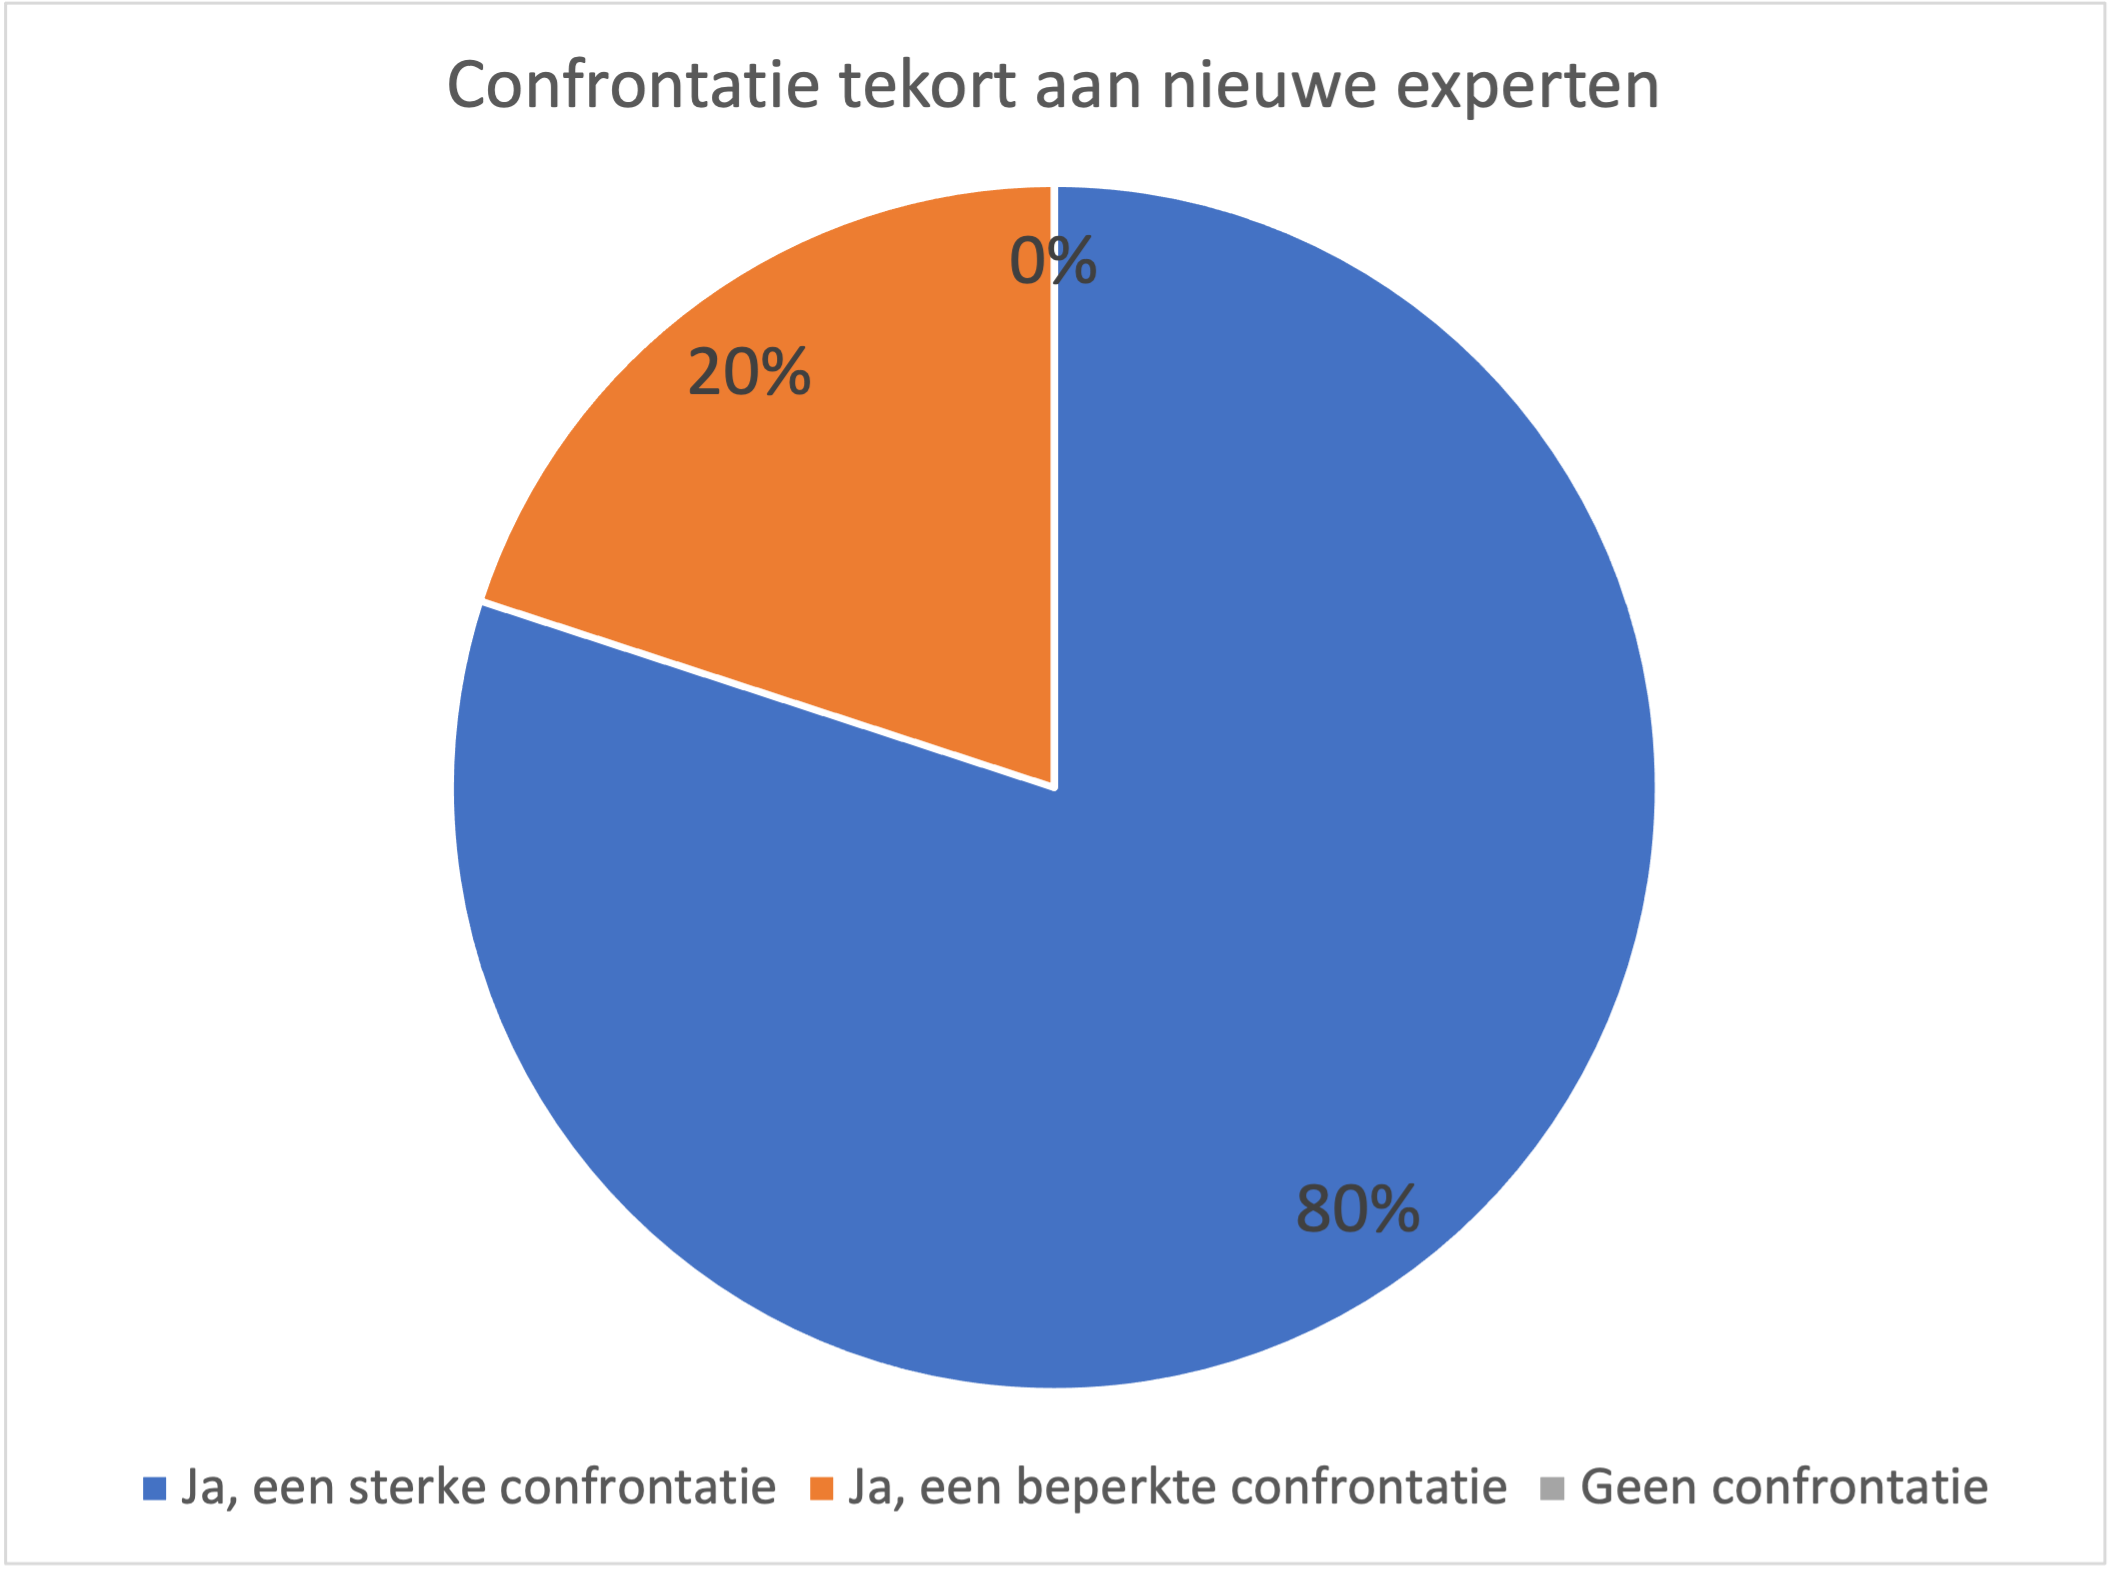
\includegraphics[width=10cm]{confront_grafiek}
     \caption{De grafiek die aangeeft hoe het is gesteld met het tekort aan mainframe-experten.}
     \label{fig: expertisetekort}
 \end{figure}

Vier bedrijven gaven duidelijk aan sterk geconfronteerd te worden met het gebrek aan nieuwe experten. Slechts één bedrijf zegt maar beperkt hiermee geconfronteerd te worden. Dat geeft een duidelijk beeld van de situatie rond het aanbod van experten op de arbeidsmarkt.

 \subsubsection{\IfLanguageName{dutch}{Wat is de visie van de bevraagde bedrijven rond expertise en welke initiatieven zetten ze hiervoor op?}{What are the questioned companies vision about expertise and what are their initiatives to handle this?}}
\label{sec:Wat is de visie van de bevraagde bedrijven rond expertise en welke initiatieve zetten ze hiervoor op?}

De organisaties hebben de vragen beantwoord naar hun visie omtrent de eerder benoemde tekorten aan nieuwe expertise. Hieruit blijkt dat er een tekort is bij alle vijf bedrijven. Daarnaast zegt één bedrijf dat het problematisch is. Als gevolg hiervan kregen ze de vraag of ze initiatieven hebben uitgewerkt om hierop in te spelen. Drie van de vijf bedrijven organiseert interne opleidingen voor huidige en nieuwe werknemers. Zij zetten eveneens in op een opleidingstraject voor nieuwe werknemers en schoolverlaters. Opmerkelijk was dat er maar één bedrijf als enige oplossing een migratie naar de cloud voor ogen had. 

\newpage

\subsubsection{\IfLanguageName{dutch}{Welke nadelen brengt het gebruik van een mainframe mee voor de organisatie?}{What are the disadvantages of a mainframe for your company?}}
\label{sec:Welke nadelen brengt het gebruik van een mainframe mee voor de organisatie?}

Op bovenstaande vraag hebben vier bedrijven een antwoord gegeven. De voornaamste nadelen die zij aankaarten zijn de volgende:
  \begin{itemize}
     \item Gelimiteerd aantal resources 
     \item Gelimiteerde grafische user interface mogelijkheden
     \item Veel legacy code 
     \item Kan huidige trends en standaarden niet bijhouden
     \item Weinig mogelijkheden in verband met web integraties
     \item Dalende expertise
     \item Beperkt in het implementeren van Agile development toepassingen
     \item Kleine teams die miljoenen batchprogramma's en online transacties dienen te onderhouden
 \end{itemize}

\subsubsection{\IfLanguageName{dutch}{Heeft de organisatie migratieplannen?}{Has your organization any migration plans?}}
\label{sec:Heeft de organisatie migratieplannen?}

 \begin{figure}[h]
    \centering
    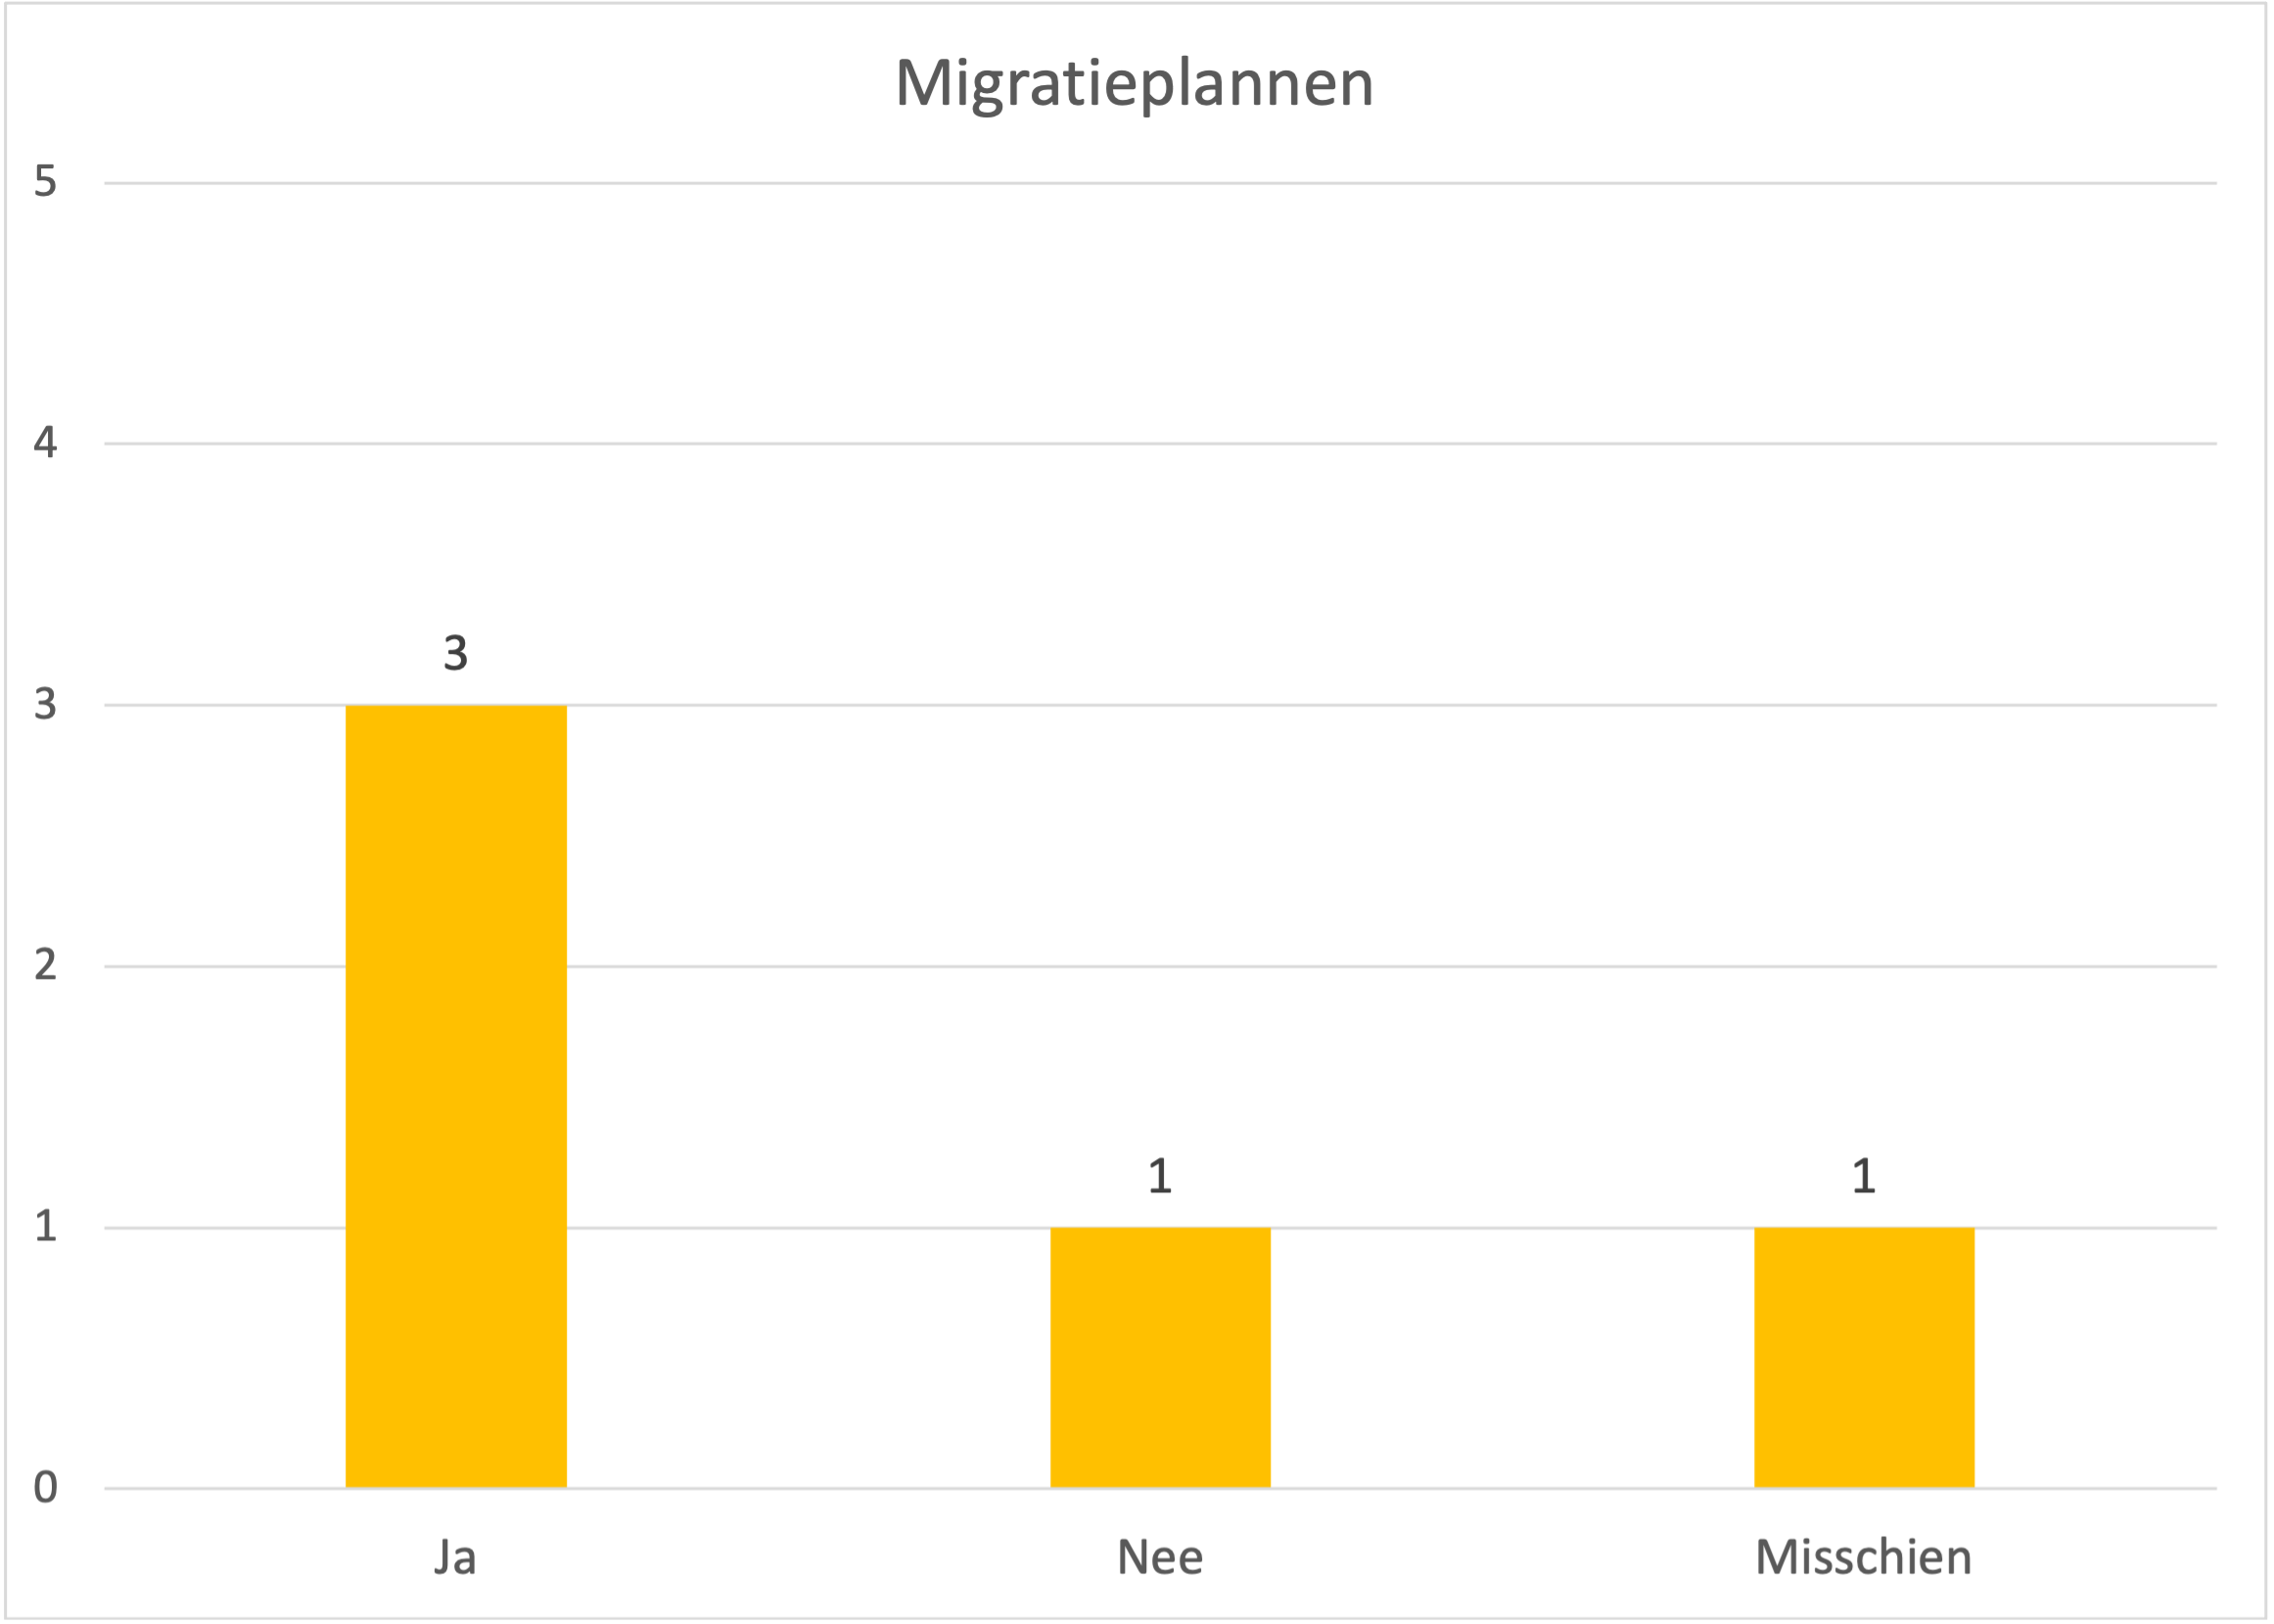
\includegraphics[width=10cm]{migratie_grafiek}
    \caption{De grafiek die aangeeft of er migratieplannen zijn.}
    \label{fig: migratieplannen}
\end{figure}


In dit onderzoek is de migratie van de mainframe workload een belangrijk onderwerp. De bedrijven die deelnamen aan de enquête hebben geantwoord op de bovenstaande vraag. Drie organisaties hebben standvast plannen om een migratie uit te voeren naar een alternatief platform zoals de cloud. Bij de andere twee is er enerzijds een zekerheid dat hun mainframe workload niet zal gemigreerd worden terwijl anderzijds bij het andere bedrijf het wordt overwogen. 

Vervolgens werd de vraag gesteld waarom ze al dan niet een migratie zouden doen. De redenen die zij aankaarten om het wel te doen is vooral de omzetting naar een layered architectuur en de kosten van een mainframeplatform die in vraag worden gesteld. Ten slotte geeft het bedrijf zonder migratieplannen aan dat de betrouwbaarheid en de impact van een migratie op hun core business een goede reden is om nooit een migratie uit te voeren. 

\newpage

\subsection{\IfLanguageName{dutch}{De resultaten van de bevragingen voor studenten en IT-professionals}{The results of the survey for students and IT-professionals}}
\label{sec:De resultaten van de bevragingen voor studenten en IT-professionals}

Aan de tweede enquête namen 12 personen deel. Er werd bevraagd waar hun interesses liggen en of zij al in contact zijn gekomen met een mainframe. Daarnaast werd bevraagd of zij zouden openstaan voor een opleiding in de wereld van mainframeontwikkeling. 

De resultaten hieronder zijn opgedeeld per vraag.

\subsubsection{\IfLanguageName{dutch}{Wat is uw functie?}{What is your function?}}
\label{sec:Wat is uw functie?}

 \begin{figure}[h]
    \centering
    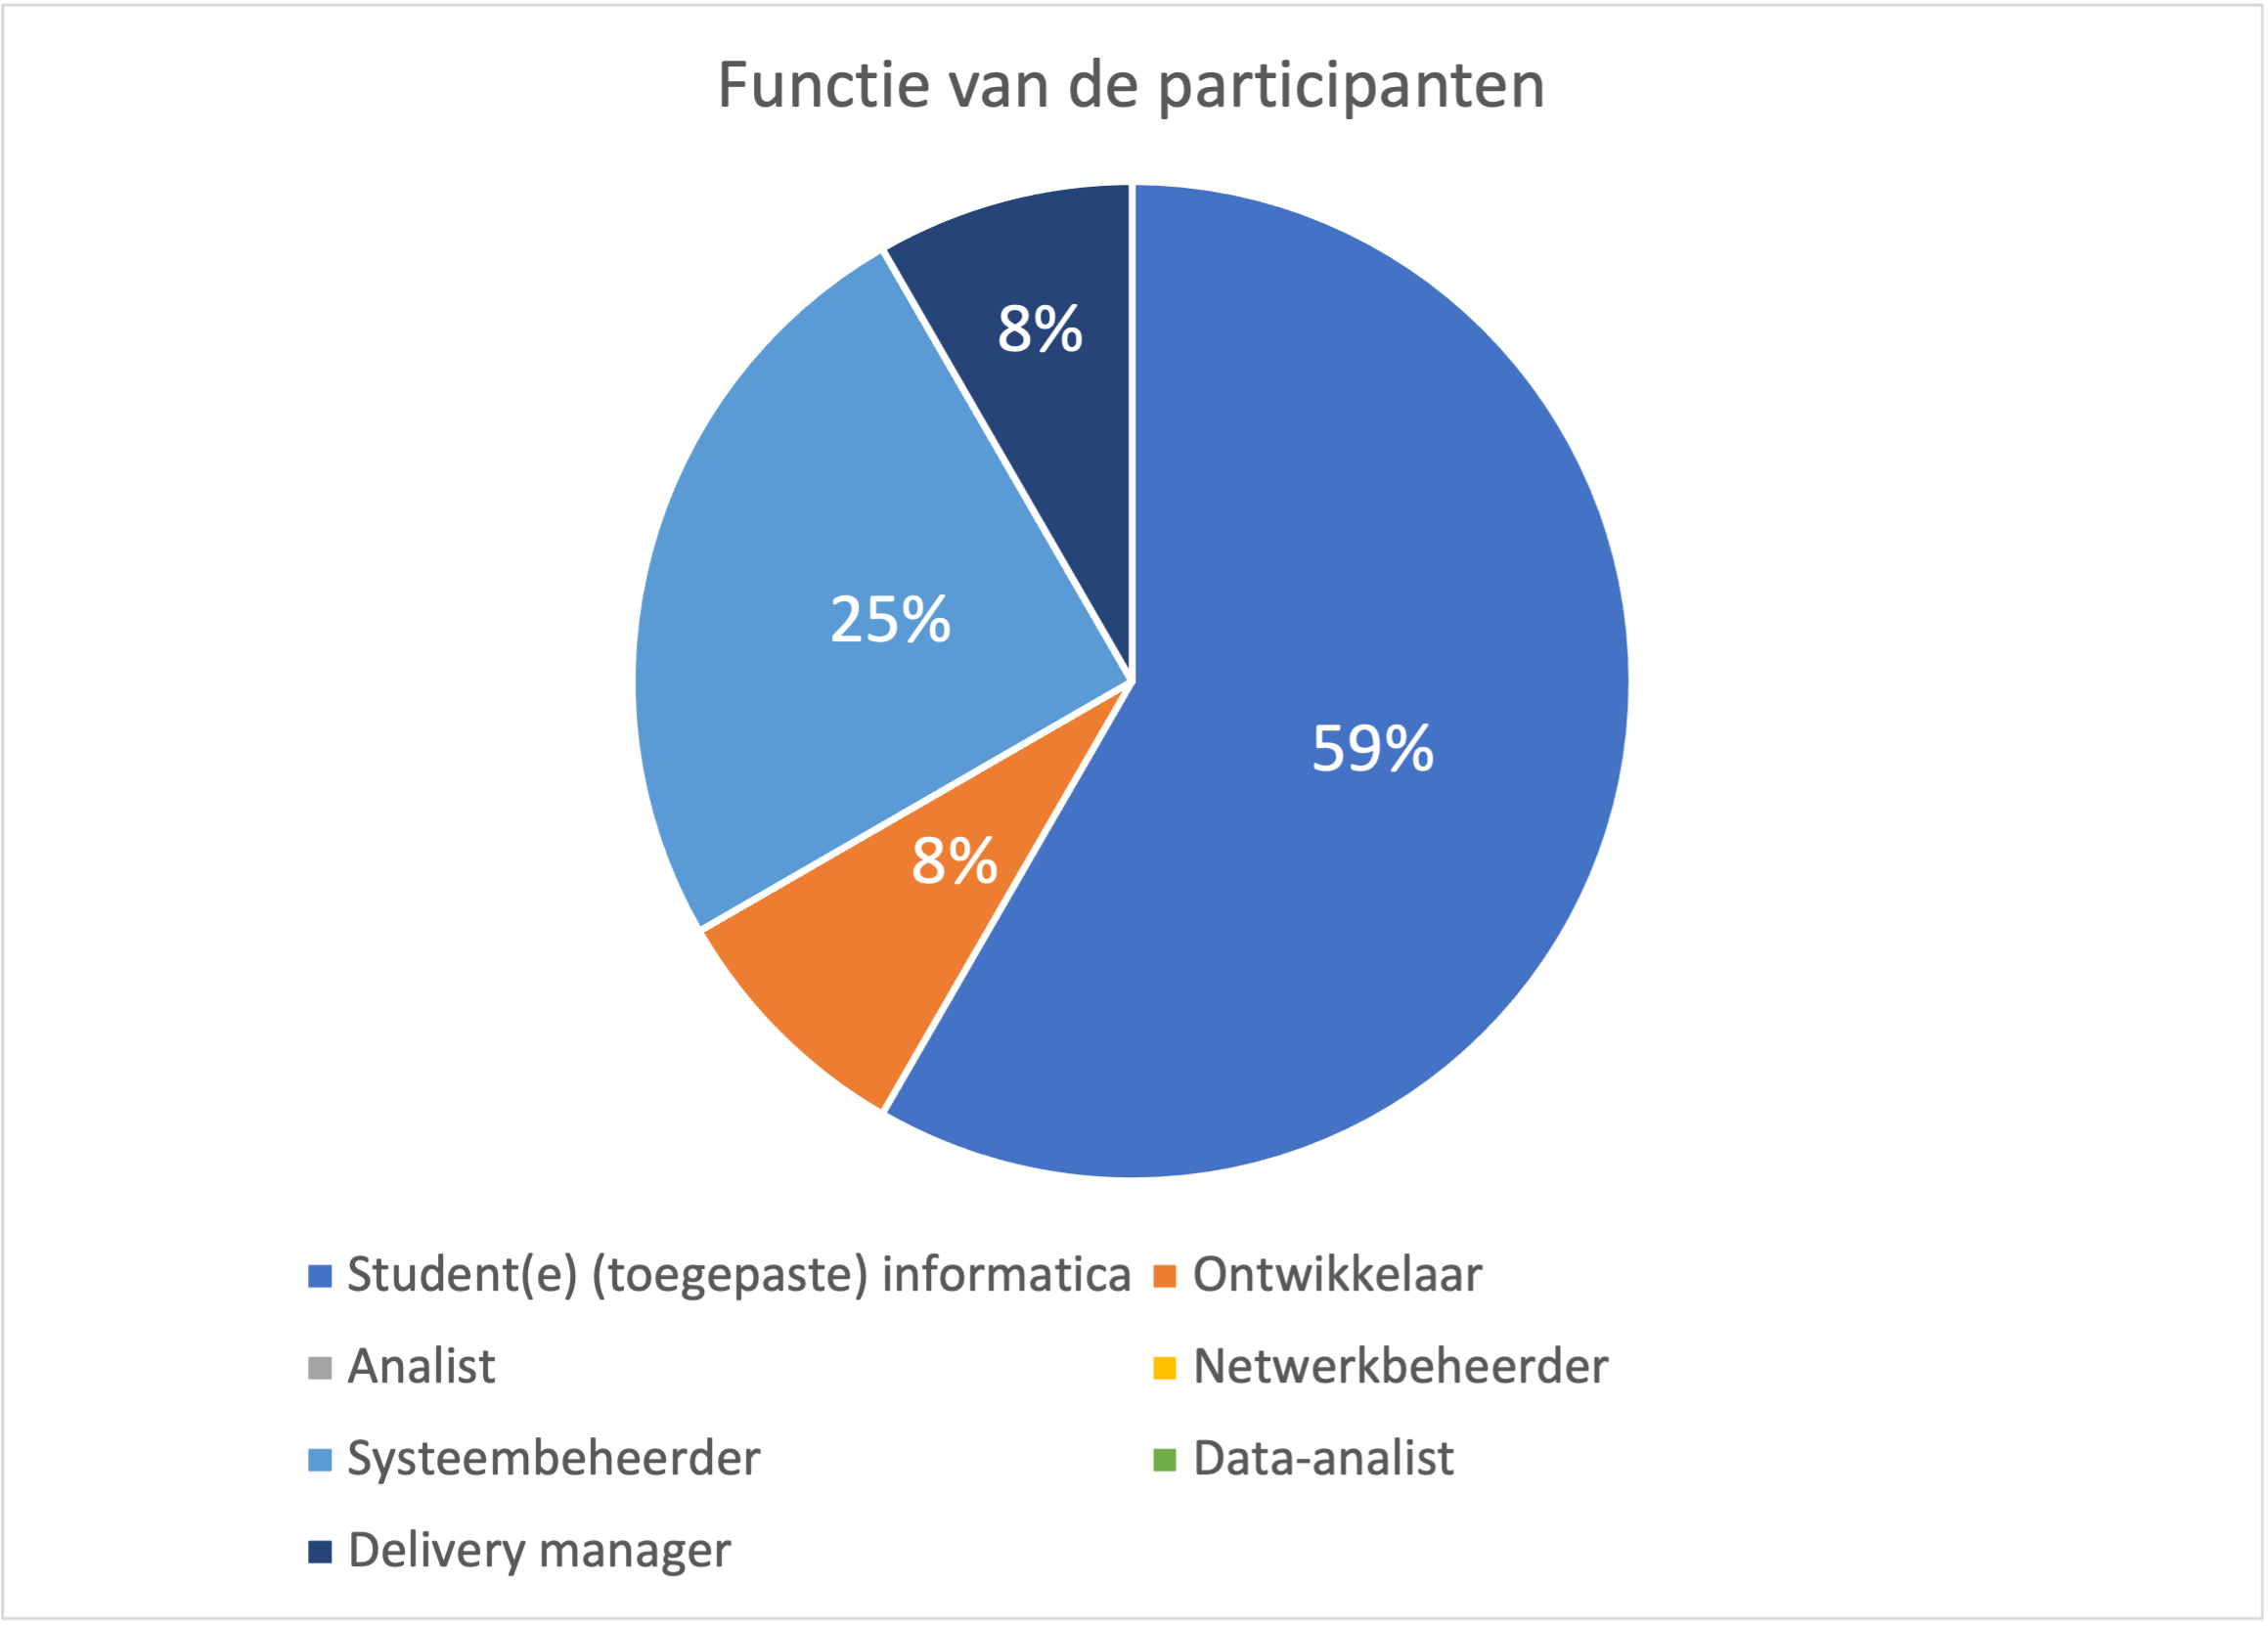
\includegraphics[width=10cm]{functie_grafiek}
    \caption{De grafiek die  de functies van de participanten representeert.}
\end{figure}

Het meeste van de kandidaten waren studenten (toegepaste) informatica. Zij vertegenwoordigde het grootste deel van de groep participanten. Onder hen waren de systeembeheerders met de meeste personen. Daarnaast nam juist één ontwikkelaar en één delivery manager deel.  

\newpage

\subsubsection{\IfLanguageName{dutch}{Wat is uw leeftijd?}{What is your age?}}
\label{sec:Wat is uw leeftijd?}

 \begin{figure}[h]
    \centering
    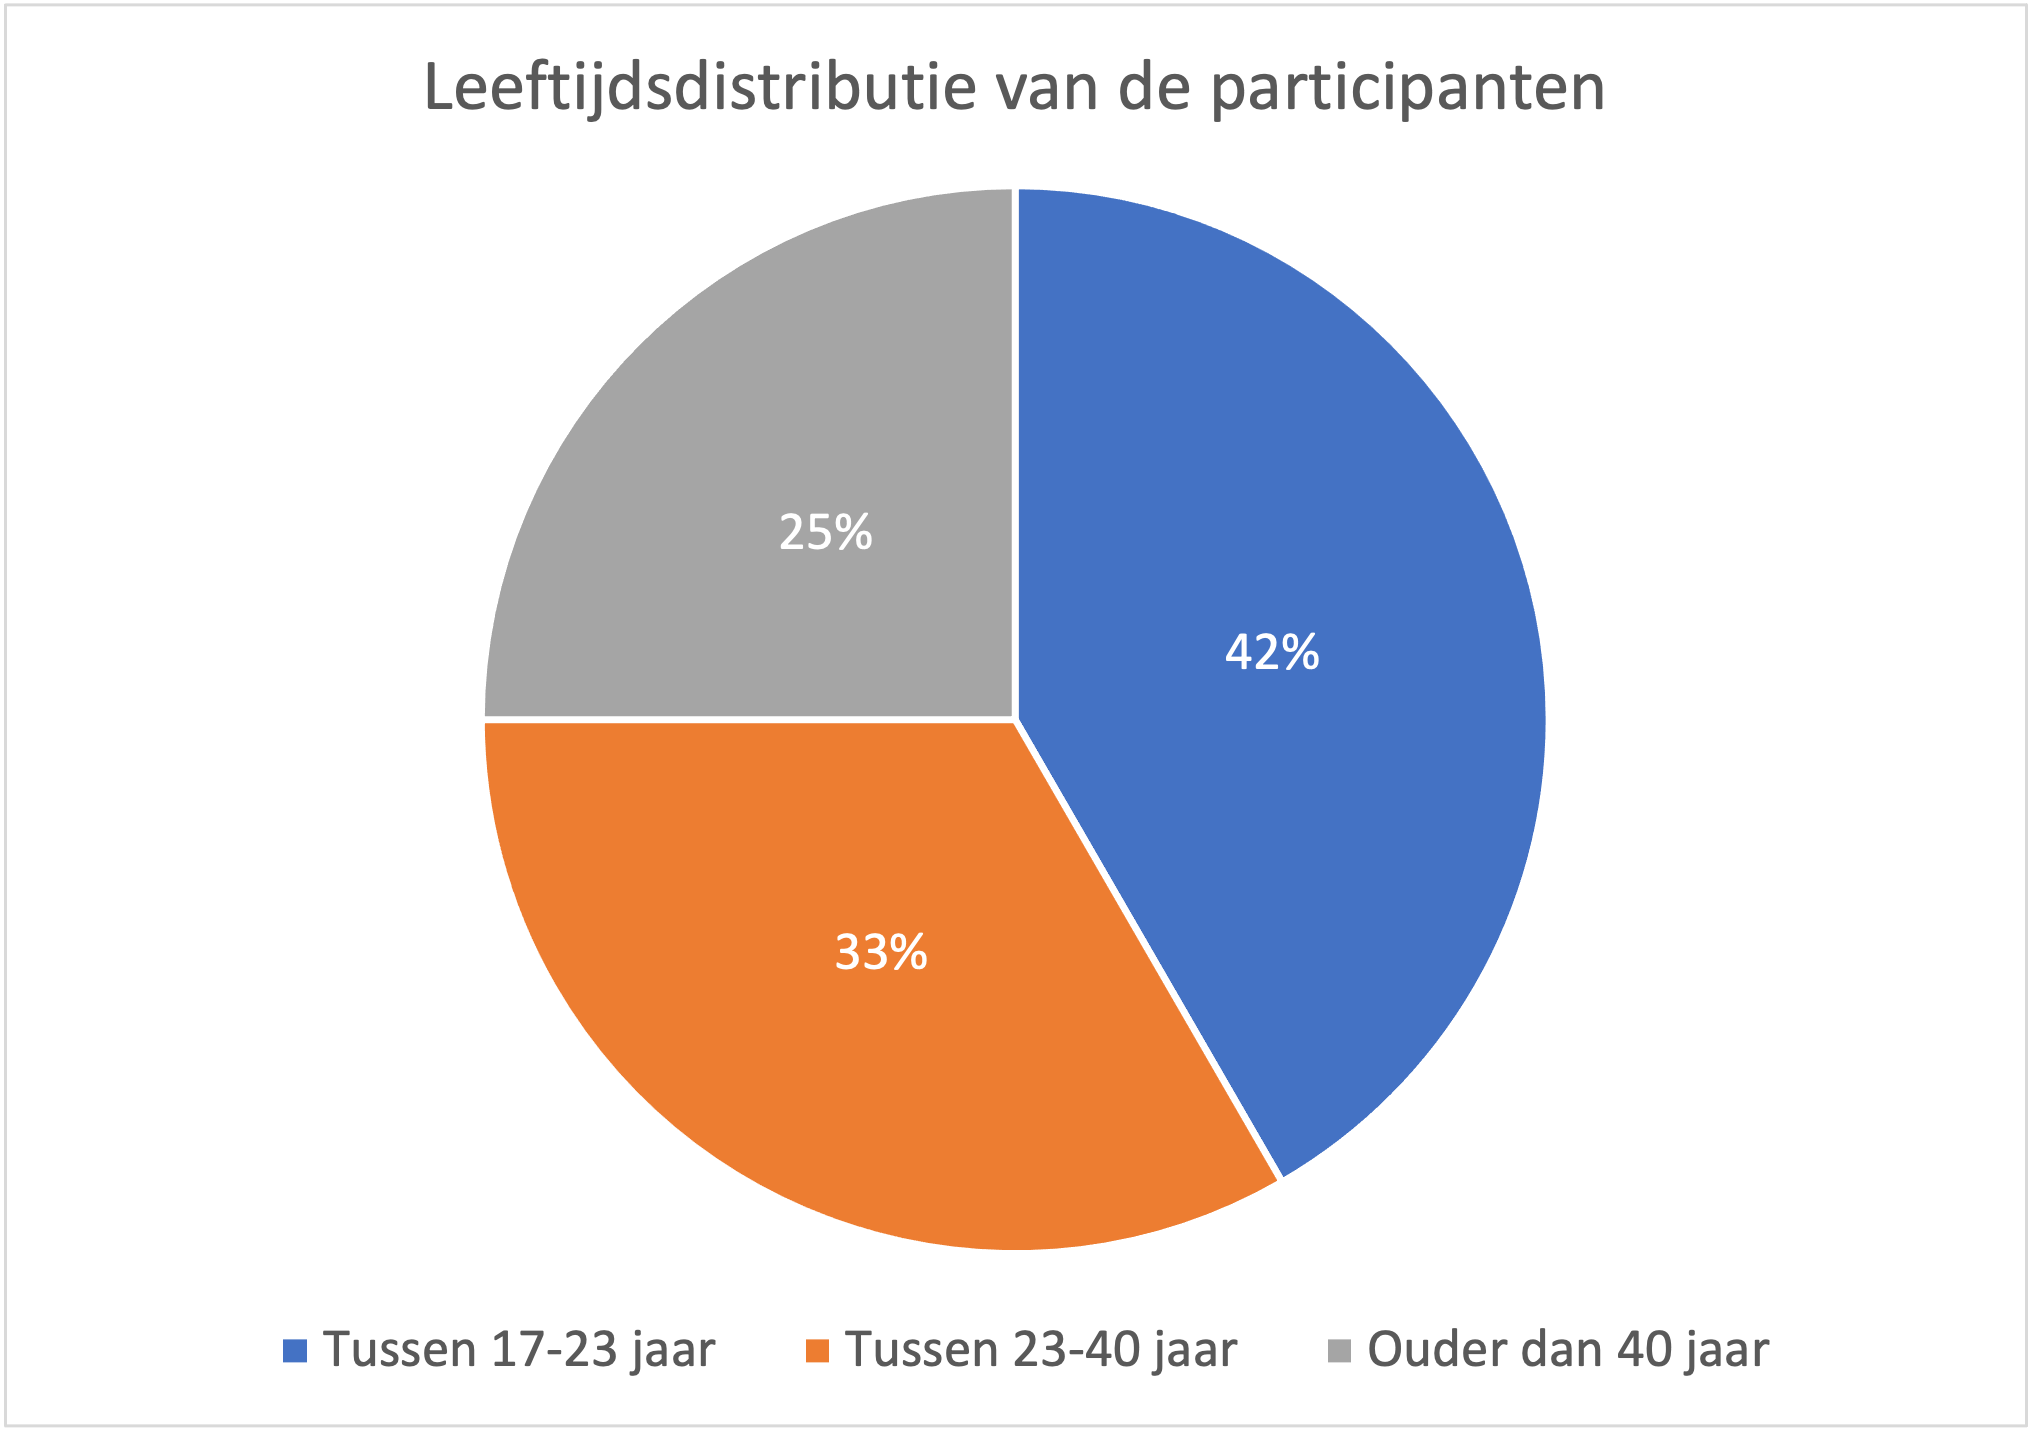
\includegraphics[width=10cm]{leeftijd_grafiek}
    \caption{De grafiek die de leeftijdsdistributie van de participanten representeert.}
\end{figure}


De leeftijdsdistributie van het onderzoek was het ideaal scenario. Er was een relatief gelijke verdeling van zowel personen die de opkomst van de mainframe hebben doorgemaakt als personen die opgeleid worden in een wereld van gedistribueerde technologieën. Dat zorgde ervoor dat de participanten hun kennis van de mainframecomputer een breed spectrum aannam. 

\subsubsection{\IfLanguageName{dutch}{Weet u wat een mainframe is?}{Do you know what a mainframe is?}}
\label{sec:Weet u wat een mainframe is?}

 \begin{figure}[h]
    \centering
    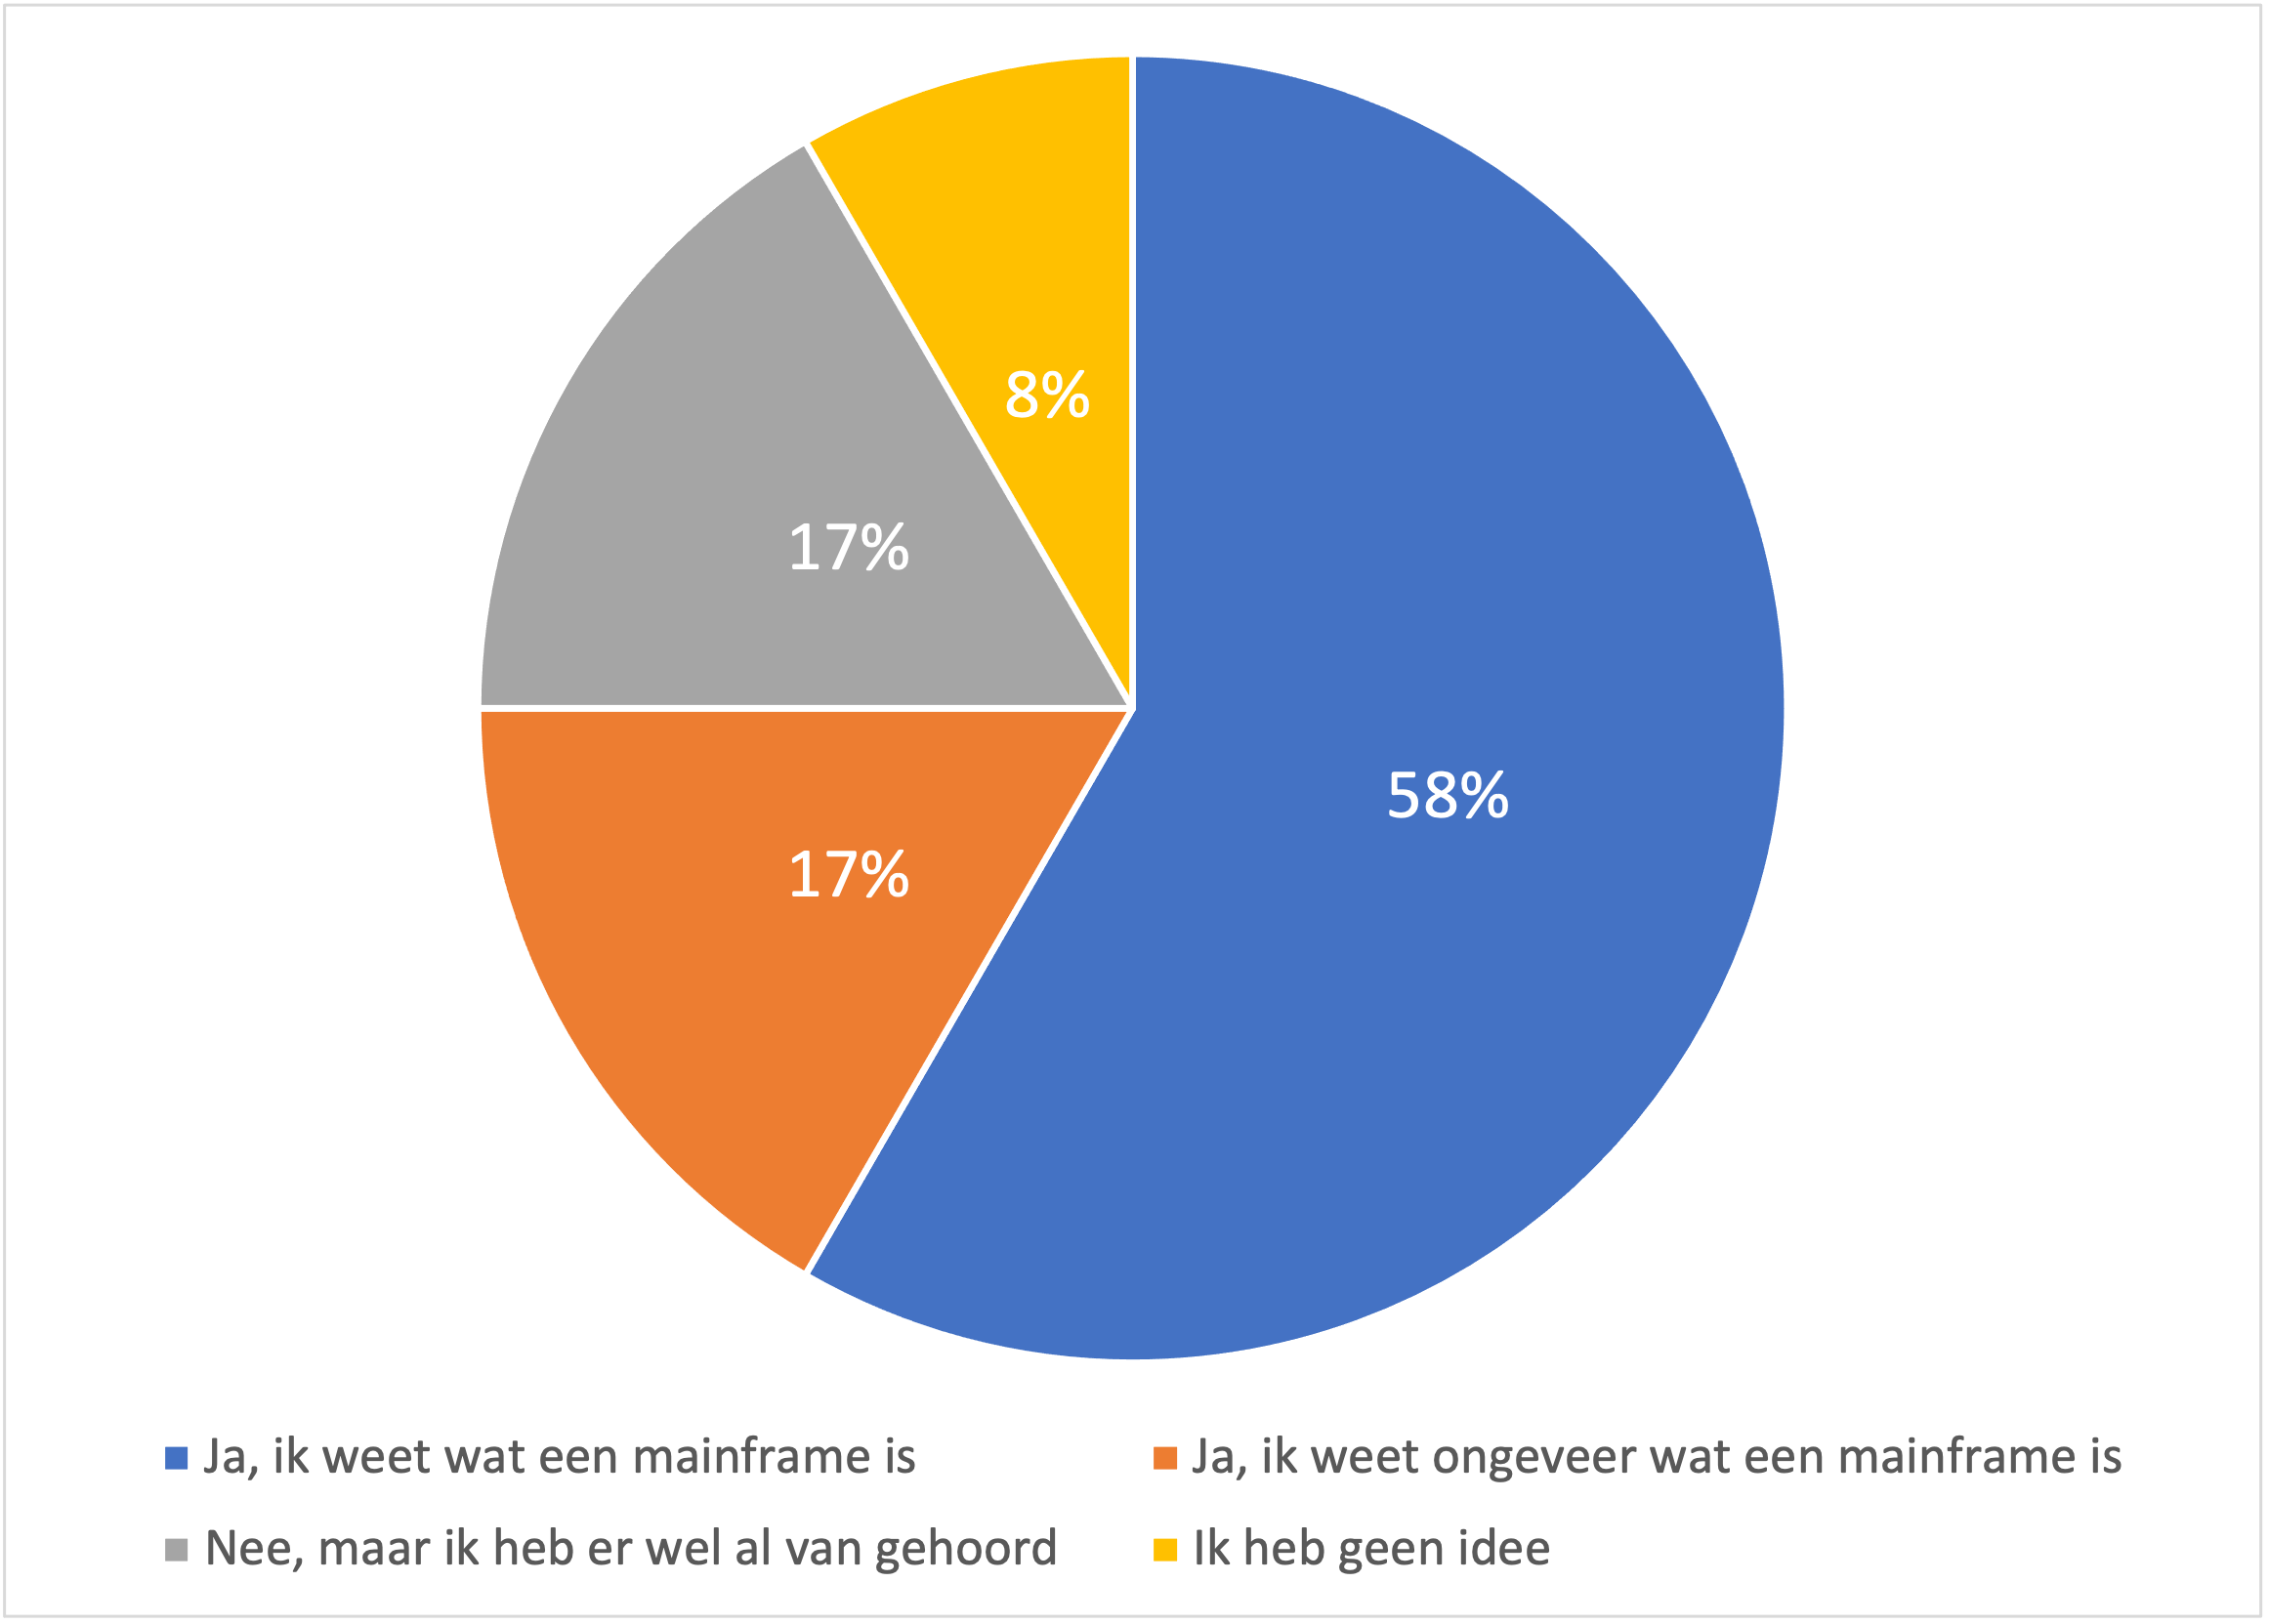
\includegraphics[width=10cm]{kennis_grafiek}
    \caption{De grafiek die aangeeft hoeveel participanten weten wat een mainframe is.}
\end{figure}

Slechts één bevraagde wist niet wat een mainframe is en zeven van de twaalf participanten wisten perfect wat een mainframe is. 

\newpage

\subsubsection{\IfLanguageName{dutch}{Heeft u ervaring of bent u al in contact geweest met de programmeertalen COBOL of PL/1?}{Do you have experience with or did you already get in touch with COBOL or PL/1?}}
\label{sec:Heeft u ervaring of bent u al in contact geweest met de programmeertalen COBOL of PL/1?}

 \begin{figure}[h]
    \centering
    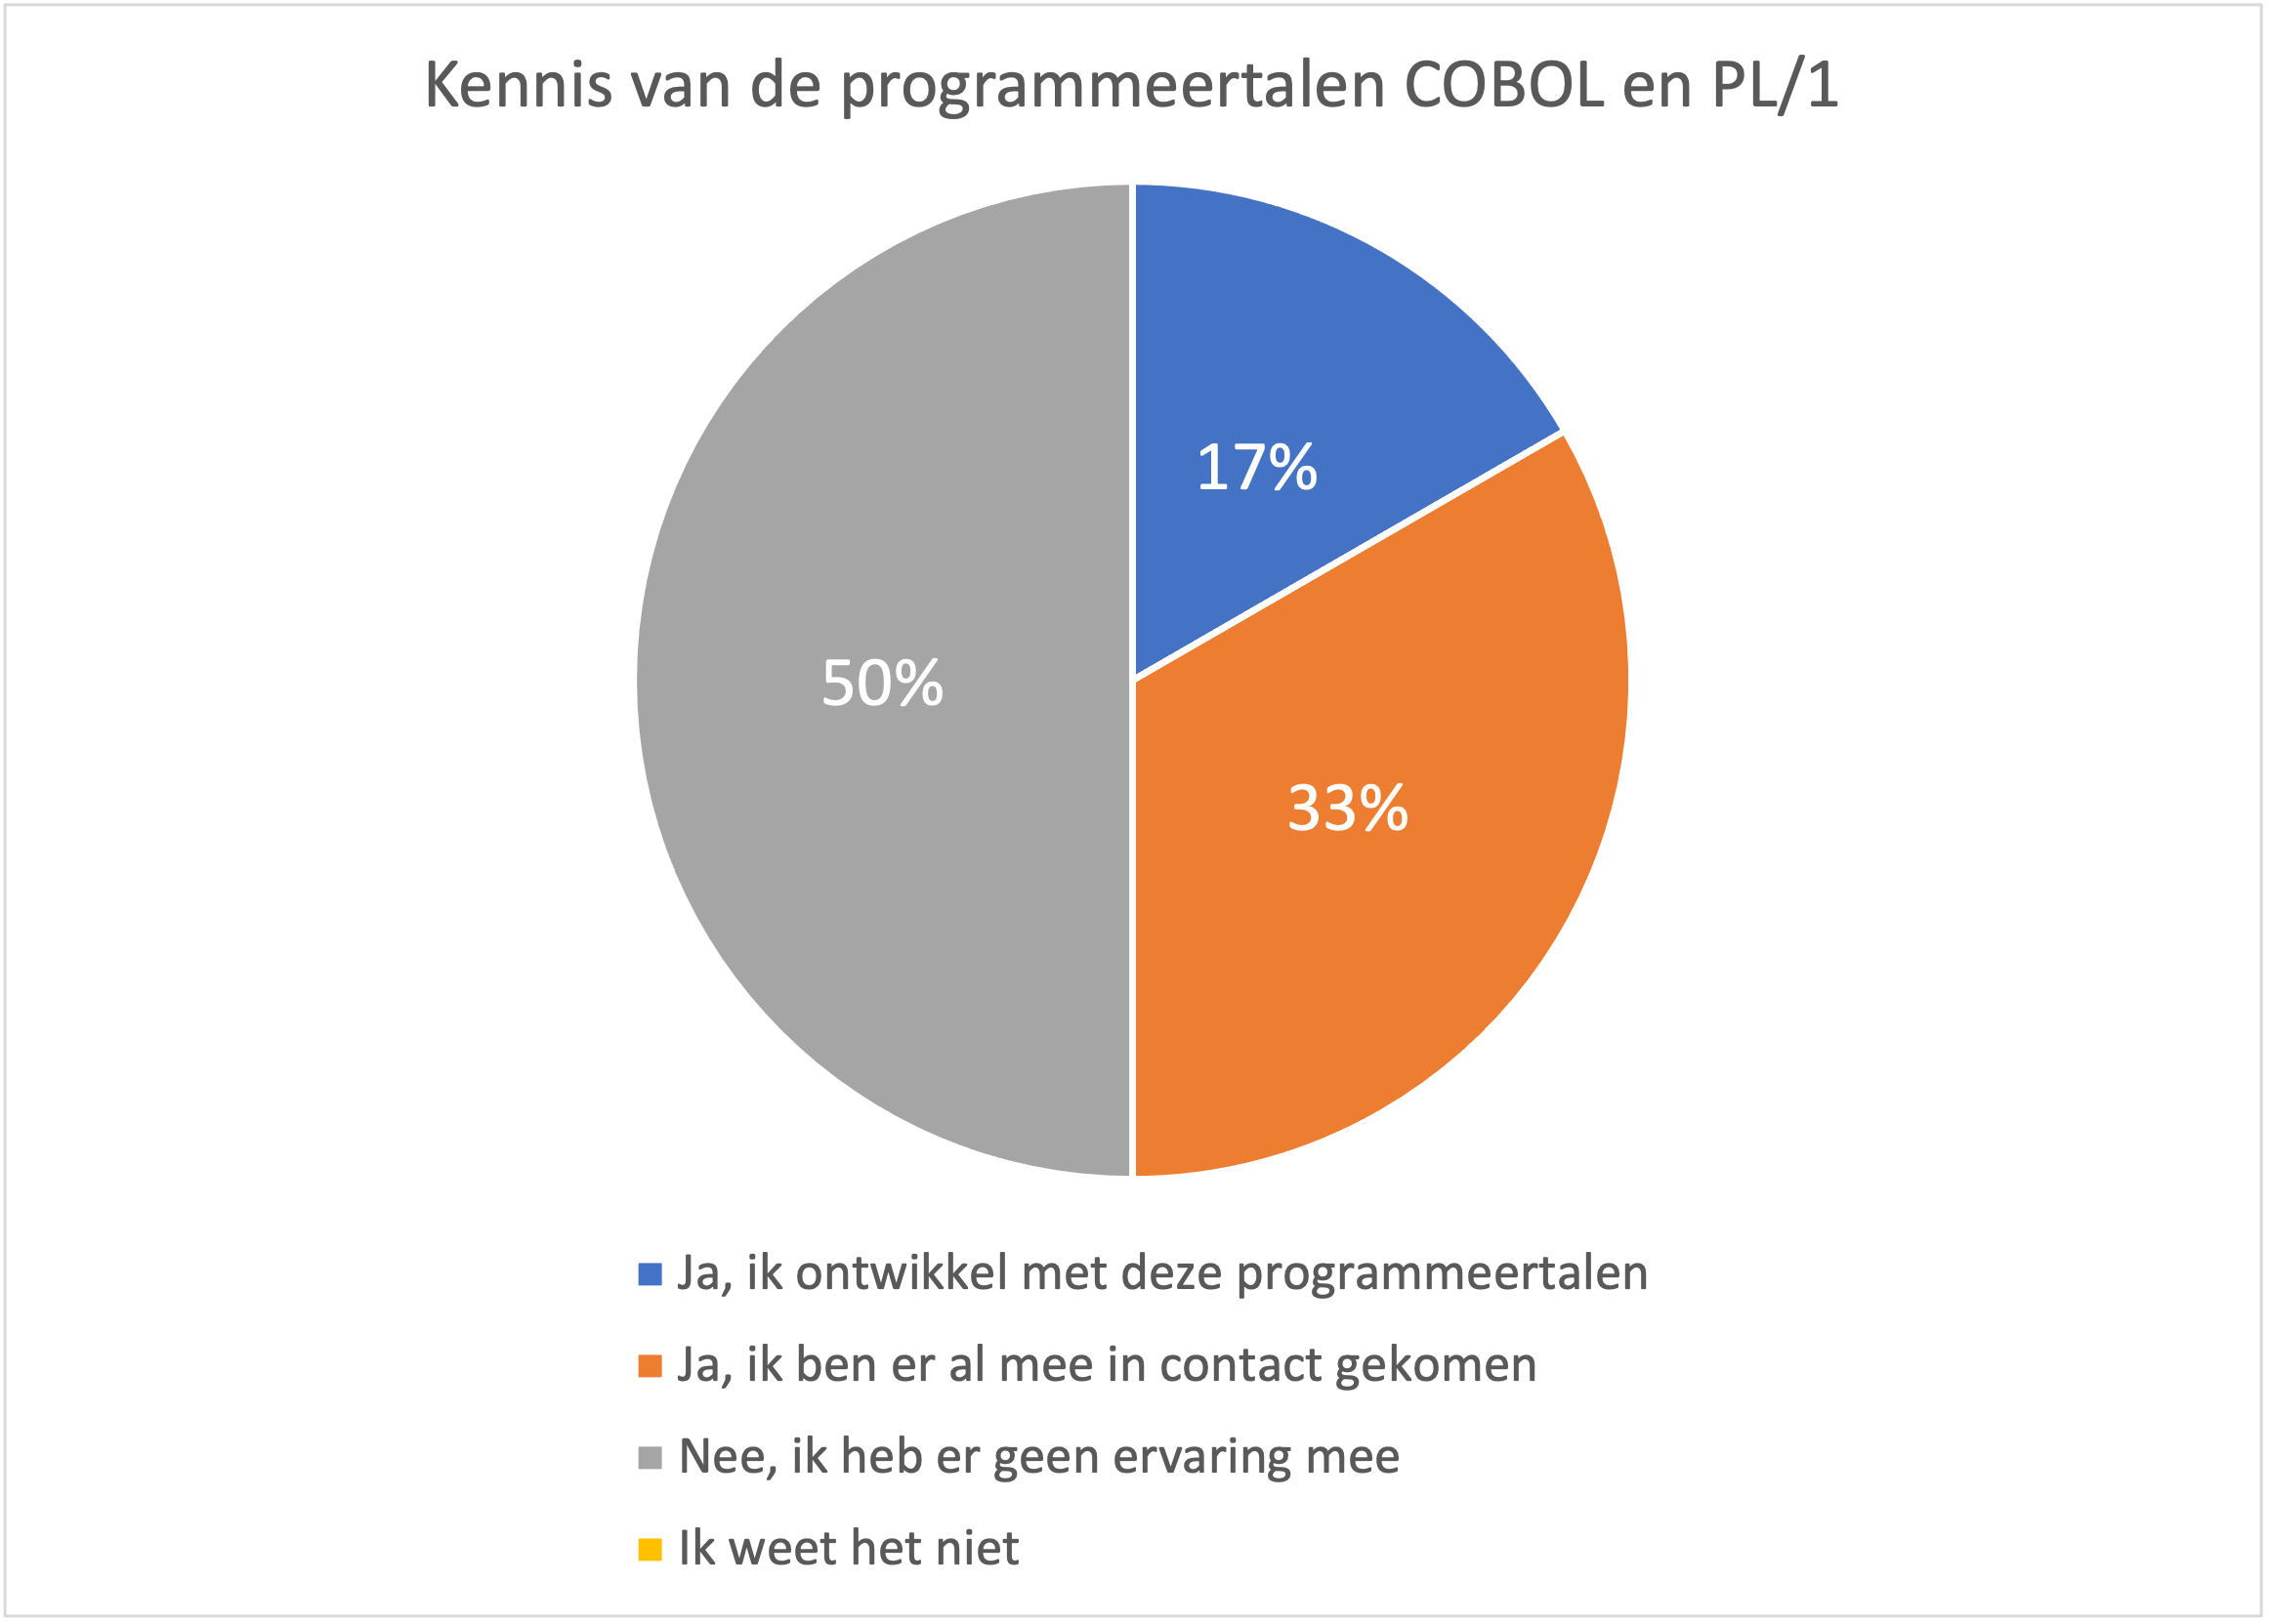
\includegraphics[width=10cm]{Progtalen_grafiek}
    \caption{De grafiek  die aangeeft welke kennis de participanten beheersen over de mainframespecifieke programmeertalen.}
\end{figure}

Twee participanten of 17\% van de participanten programmeren met de programmeertalen COBOL en PL/1. Echter gaf 50\% aan nog nooit in contact te zijn geweest met deze programmeertalen. 

Vervolgens is er in dit onderzoek bevraagd hoe het zat bij de interesses van de participanten. Uit de bevraging moest duidelijk zijn of een opleiding in de mainframewereld nog aantrekkelijk is voor de hedendaagse studenten. Hieronder bevinden zich twee grafieken met de antwoorden op volgende vragen:
  \begin{itemize}
    \item Zou u geïnteresseerd zijn om COBOL of PL/1 te studeren?
    \item Zou u kiezen voor een opleiding als mainframe-expert?
\end{itemize}

\begin{figure}[h]
    \centering
    \begin{subfigure}{0.45\textwidth}
        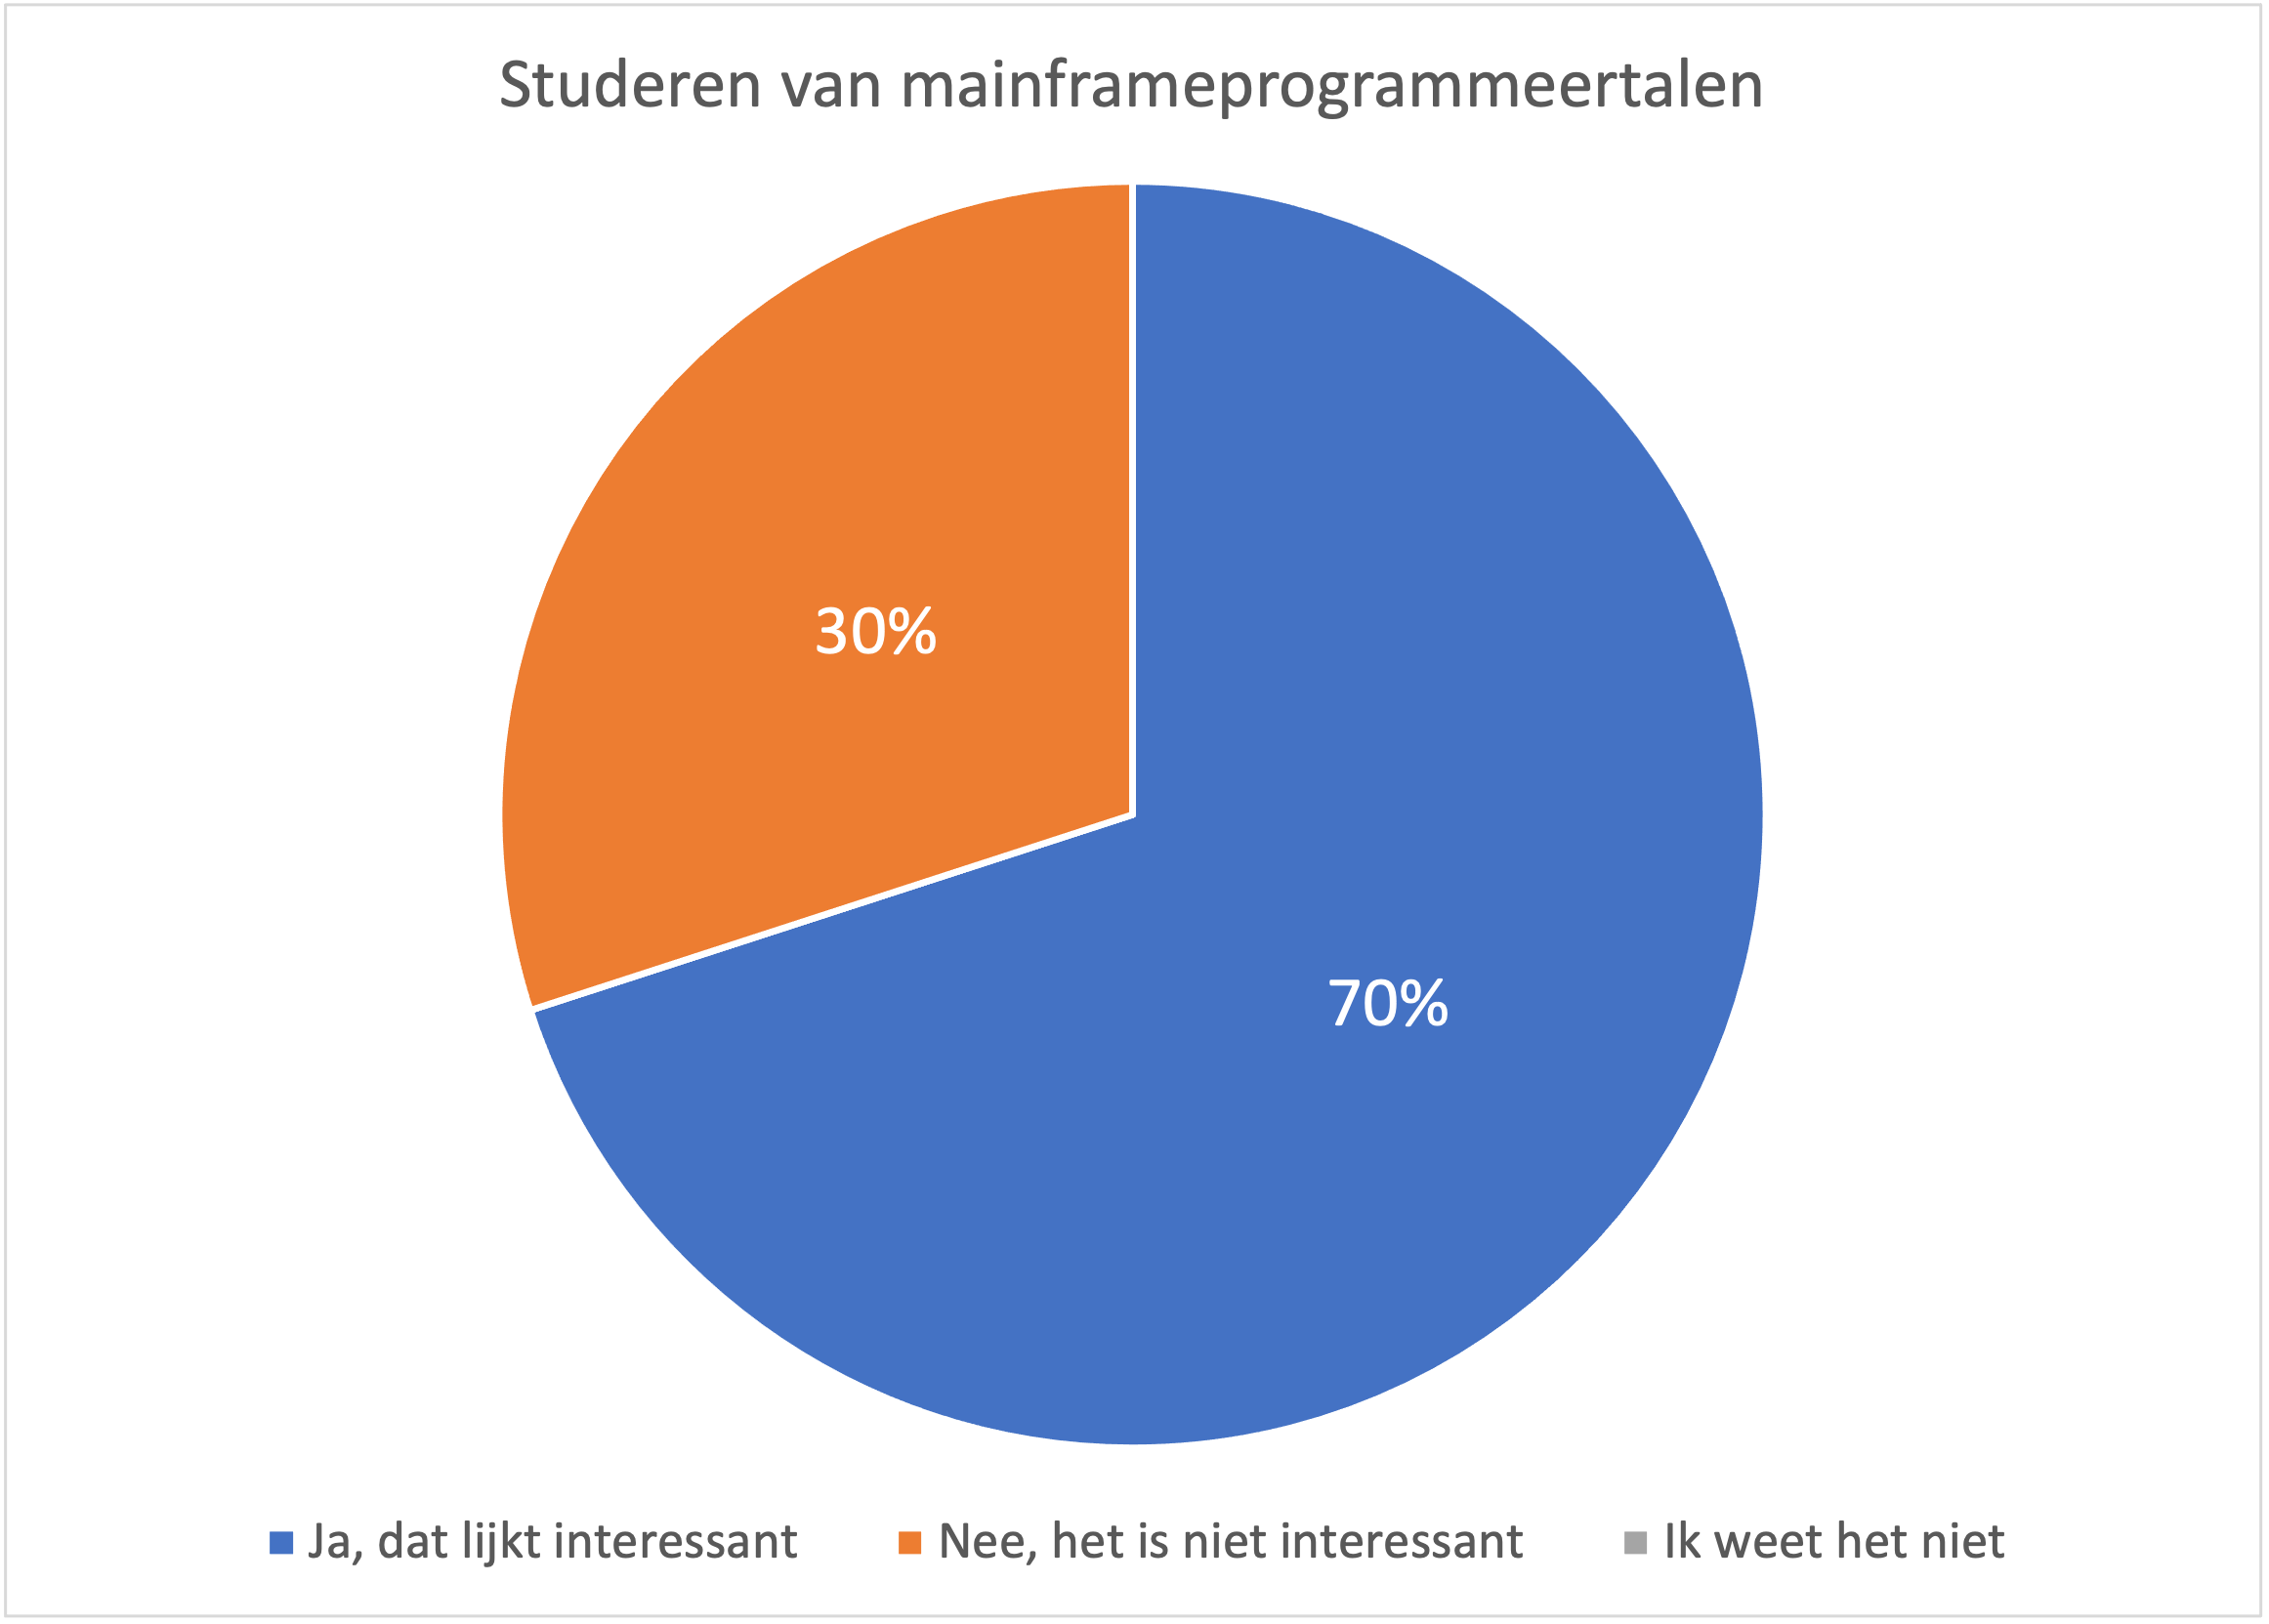
\includegraphics[width=\textwidth]{stud_grafiek}
        \caption{De grafiek die aangeeft hoeveel participanten mainframeprogrammeertalen zouden willen studeren.}
        \label{fig:studeren}
    \end{subfigure}
    \hfill
    \begin{subfigure}{0.45\textwidth}
        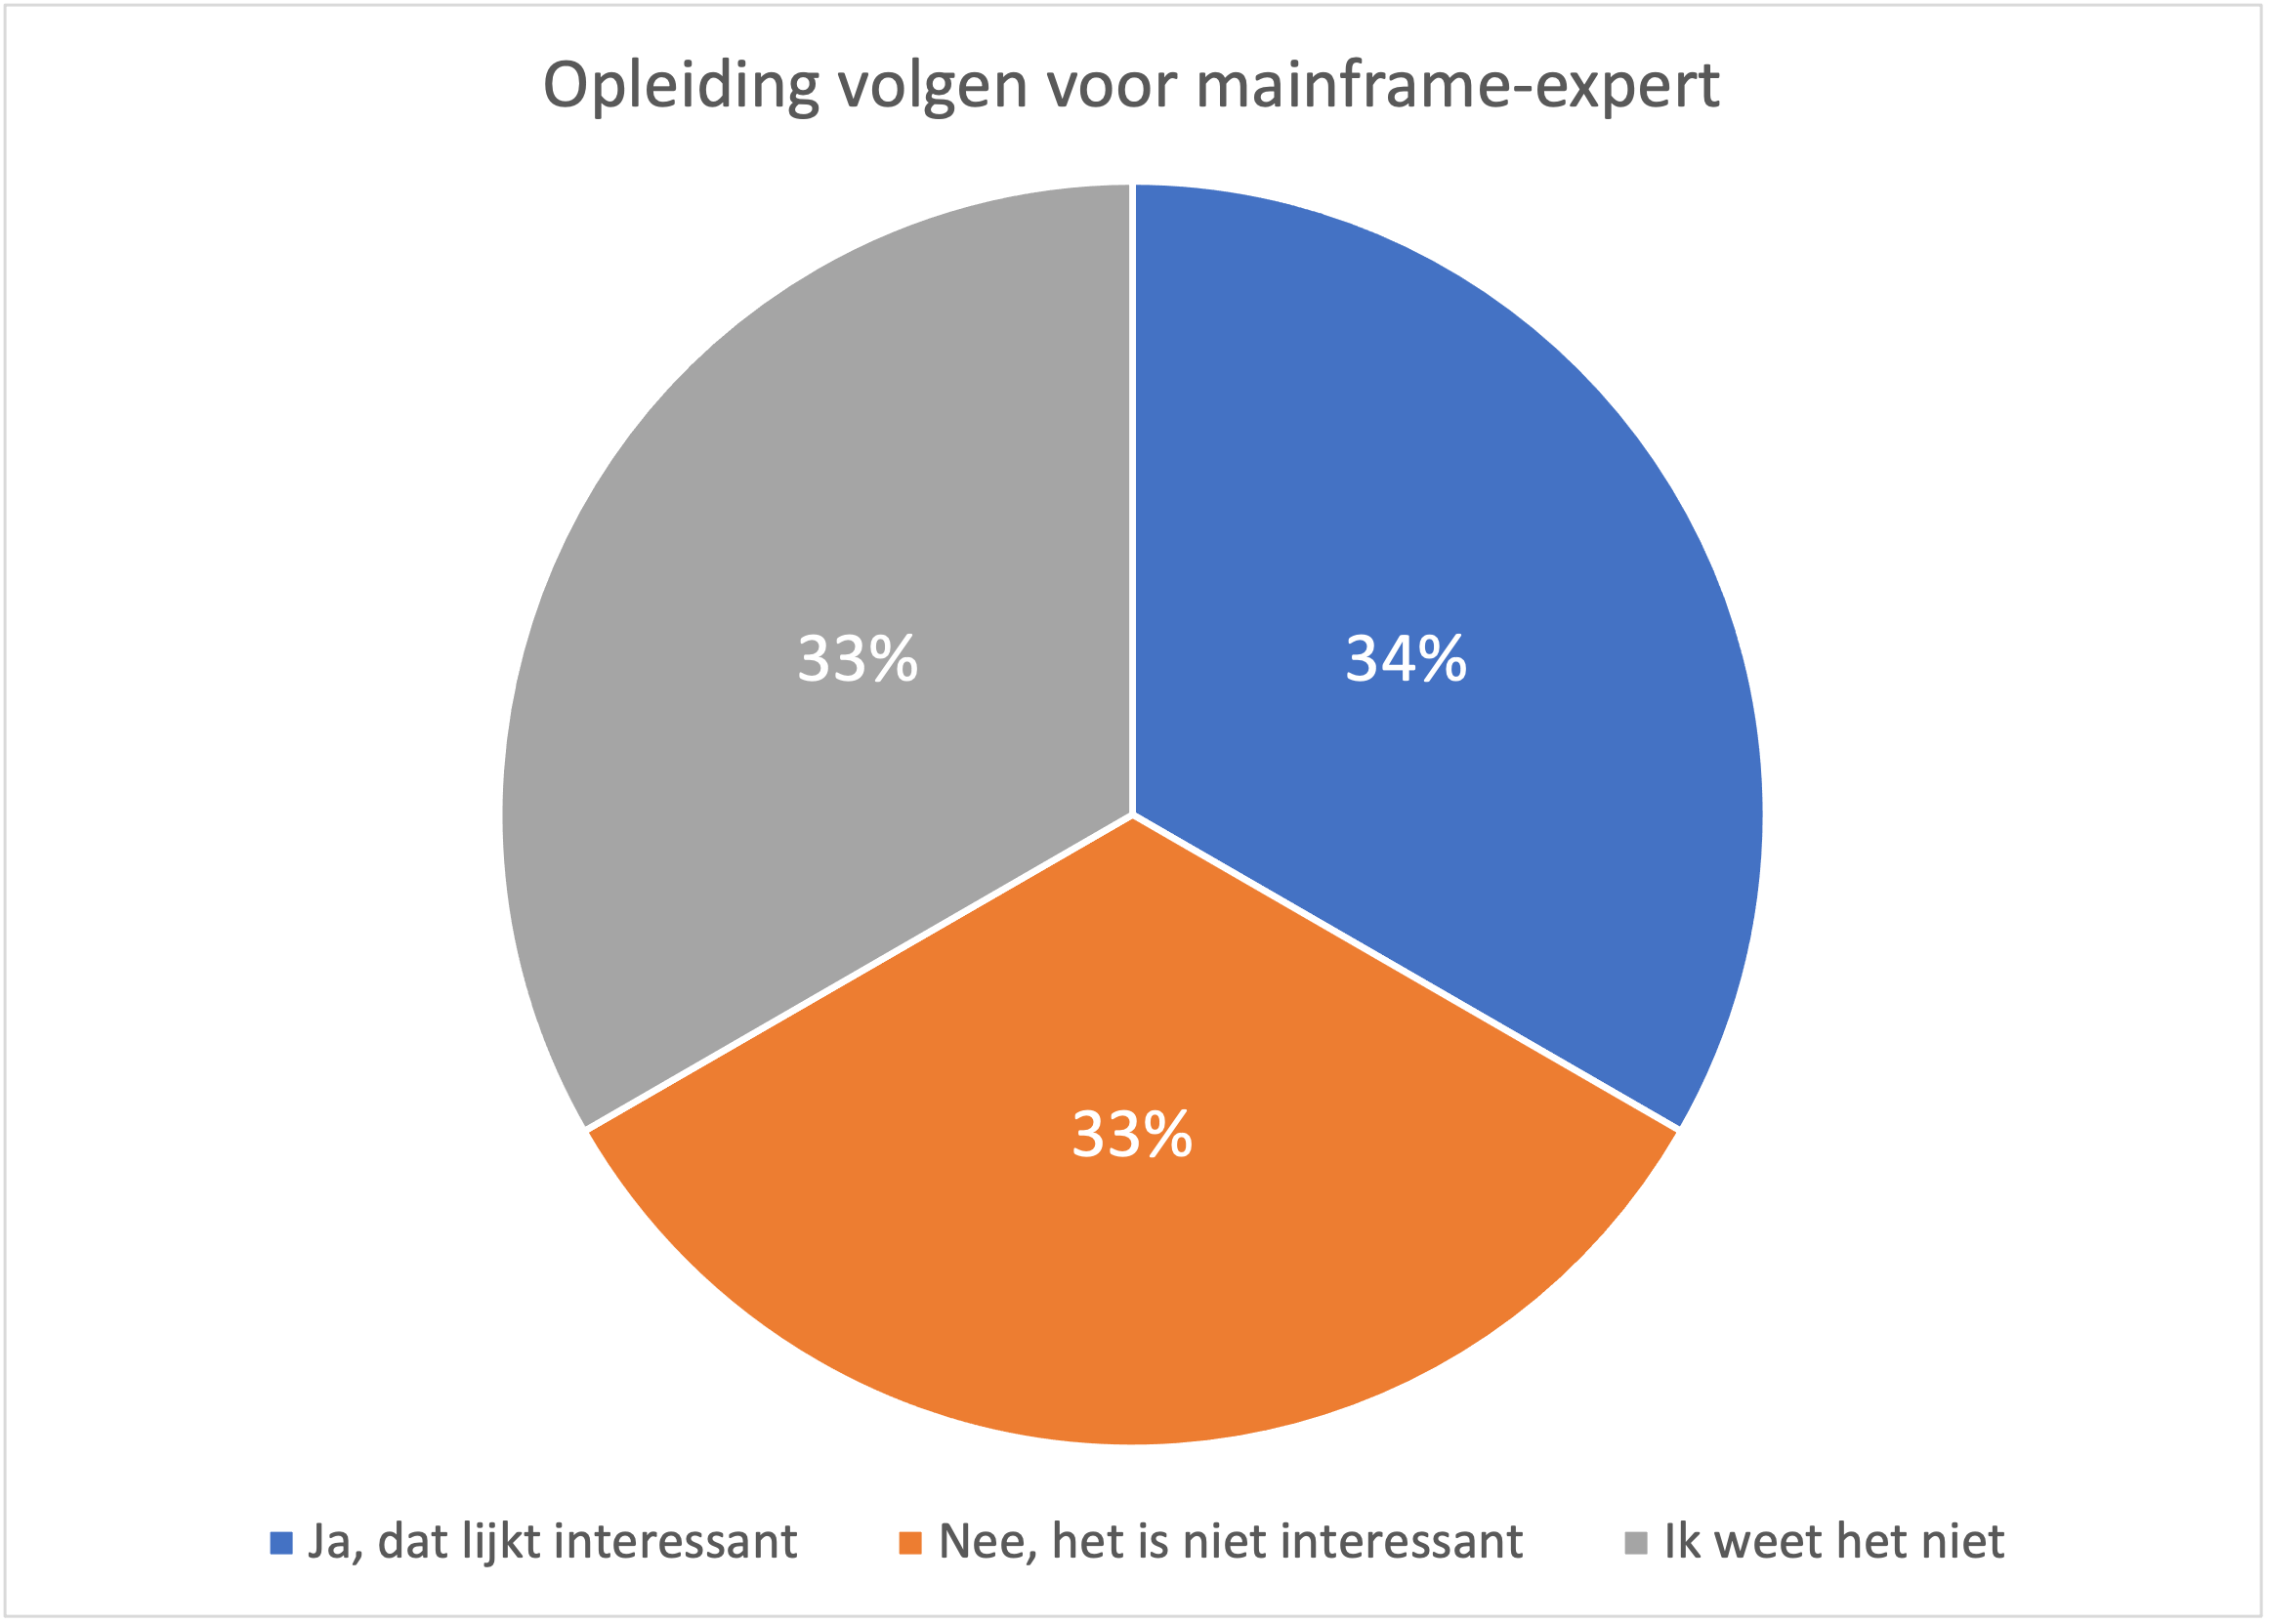
\includegraphics[width=\textwidth]{op_grafiek}
        \caption{De grafiek die aangeeft hoeveel participanten de opleiding van mainframe-expert zouden volgen.}
        \label{fig:opleiding}
    \end{subfigure}
\end{figure}



